% Created 2024-03-11 Mo 11:12
% Intended LaTeX compiler: pdflatex
\documentclass[aspectratio=169]{beamer}
% \usepackage{euler}
\usepackage{ifthen}
% \usepackage{my-defs}
\usepackage{amsmath}
\usepackage{textcomp}
\usepackage{amssymb}
\usepackage{comment}
\usepackage{booktabs}
\usepackage{fontawesome5}
\AtBeginSection[]{\begin{frame}<beamer>\frametitle{Topic}\tableofcontents[currentsection]\end{frame}}

\usepackage{proof} \usepackage{tikz}
\newcommand{\chr}[1]{{\color{blue}#1}}
\def\maxcon{\mathsf{maxcon}}
\def\states{\mbox{\color{black!50}\footnotesize \faBullhorn}} \def\saw{\mbox{\color{black!50}\footnotesize \faEye}}
\newcommand{\SAW}[2]{\saw_{#1}^{\sf rel}#2} \newcommand{\STATES}[2]{\states_{#1}^{\sf rel}#2}
\def\sis{\mathsf{sis}} \def\bro{\mathsf{bro}} \def\Cha{\mathsf{Cha}} \def\Norbert{\mathsf{Nor}} \def\Albert{\mathsf{Alb}} \def\king{\mathsf{king}}
\newcommand{\afnode}[3]{\fcolorbox{black}{white}{\ensuremath{#1}}\\\ensuremath{\array{c}#2\\\Rightarrow \:\: #3\endarray}} \newcommand{\afnodeH}[4]{\fcolorbox{black}{white}{\ensuremath{#1}}\\\ensuremath{#2\:\Rightarrow_{#3} \: #4}} \newcommand{\afnodeHH}[4]{\fcolorbox{black}{white}{\ensuremath{#1}}\\\ensuremath{\substack{#2\\\Rightarrow_{#3} \: #4}}}  \newcommand{\afnodeflat}[3]{\fcolorbox{black}{white}{\ensuremath{#1}}\\\ensuremath{#2 \:\Rightarrow\: #3}}  \newcommand{\afnodenoo}[3]{\ensuremath{#2 \Rightarrow #3}} \newcommand{\afnodeno}[3]{\ensuremath{\array{c}#2\\\Rightarrow \:\: #3\endarray}}
\newcommand{\afnodee}[3]{\ensuremath{#1{:}}\,\ensuremath{\left[\array{c}#2\endarray\right]}\\$~~{\Rightarrow}$\,\ensuremath{#3}}
\newcommand{\afnodeee}[3]{\ensuremath{#1{:}}\,\ensuremath{\left[\array{c}#2\endarray\right]\Rightarrow}\\\ensuremath{#3}}
\newcommand{\afnodum}[3]{\ensuremath{#1}}
\tikzstyle{os} = [draw=green!50!black,rectangle, rounded corners, minimum size=1.8em, inner sep=2pt, fill=green!15, thick, align=center]
\tikzstyle{ospale} = [draw=black!20,rectangle, rounded corners, minimum size=1.8em, inner sep=2pt, fill=white, thick, align=center]
\tikzstyle{dirdef} = [thick, red, >=latex'] \tikzstyle{def} = [thick, red, >=latex',dashed] \tikzstyle{condef} = [thick, red, >=latex', dotted]
\tikzstyle{rebut} = [thick, red, >=latex', dash dot]
\tikzstyle{attdum} = [line width=0pt, white, -] \tikzstyle{att} = [ultra thick, red, >=latex'] \tikzstyle{defaultarr} = [double, black, >=latex']  \tikzstyle{n} = [draw=black,ellipse,minimum size=1.8em, inner sep=1pt, fill=black!15, thick] \tikzstyle{na} = [draw=blue,ellipse,minimum size=1.8em, inner sep=1pt, fill=green!20, thick] \tikzstyle{ns} = [draw=red,ellipse,minimum size=1.8em, inner sep=1pt, fill=red!20, thick]  \tikzstyle{no} = [draw=blue,ellipse,minimum size=1.8em, inner sep=1pt, fill=orange!20, thick] \tikzstyle{nb} = [draw=blue,ellipse,minimum size=1.8em, inner sep=1pt, fill=blue!20, thick] \usetikzlibrary{snakes,shapes.geometric,backgrounds,calc,trees,matrix,decorations.pathmorphing,shapes,arrows,fit,backgrounds,calc,shapes.callouts,decorations.pathmorphing,arrows,decorations.markings, positioning,mindmap,backgrounds,matrix,decorations.pathmorphing,mindmap,shapes,arrows,fit,backgrounds}
\usepackage{lettrine} \usepackage{GoudyIn} \usepackage{bussproofs} \usepackage[babel=true]{csquotes}  \EnableBpAbbreviations % \usepackage{biblatex}  
\renewcommand{\LettrineFontHook}{\color{fairytalecolor}\GoudyInfamily{}} \LettrineTextFont{\itshape} \setcounter{DefaultLines}{2} %
% \addbibresource{bib.bib}
\usepackage[most]{tcolorbox} \definecolor{background}{HTML}{E6DCB8} \definecolor{linecolor}{HTML}{581810} \definecolor{fairytalecolor}{HTML}{D0220A}  % FCF9EE
\newtcolorbox{dungeonbox}{enhanced,
boxsep=0.25ex,
arc=0mm,
borderline west={1pt}{-0.5pt}{linecolor},
borderline east={1pt}{-0.5pt}{linecolor},
colback=background,
colframe=background,
overlay={
\foreach \n in {north east,north west,south east,south west}
{%
\draw [linecolor, fill=linecolor] (frame.\n) circle (2pt);
};
}
}
\newtcolorbox{argbox}{enhanced,
boxsep=0.25ex,
arc=0mm,
borderline west={1pt}{-0.5pt}{green!50!black},
borderline east={1pt}{-0.5pt}{green!50!black},
colback=green!5!background,
colframe=green!5!background,
overlay={
\foreach \n in {north east,north west,south east,south west}
{%
\draw [green!50!black, fill=green!50!black] (frame.\n) circle (2pt);
};
}
}
\newcommand*\circled[1]{\tikz[baseline=(char.base)]{             \node[shape=circle,draw,inner sep=2pt] (char) {#1};}} \newcommand*\circledfilled[1]{\tikz[baseline=(char.base)]{             \node[shape=circle,draw,inner sep=2pt, fill=black!40] (char) {#1};}}
\def\remember#1#2{%
\tcbox[enhanced,remember as={#1},frame hidden,interior hidden,boxrule=0pt,nobeforeafter,
tcbox raise base,shrink tight]{#2}%
\pgfkeyssetvalue{/myremember/#1}{#2}%
}
\def\highlighton<#1>#2{%
\alt<#1>{\tikz[overlay,remember picture]\node at (#2){%
\tcbox[enhanced,boxrule=0pt,colback=red!50,interior style={opacity=0.7},
frame style={opacity=0.5},nobeforeafter,tcbox raise base,shrink tight,
extrude by=5mm]{\pgfkeysvalueof{/myremember/#2}}};}{}%
}
\def\nor{n} \def\al{a} \newcommand{\pipenode}[2]{{\it \footnotesize #1}\\[-.4em] {\bf \color{blue} #2} }
\newtcolorbox{definitionbox}{colback=green!5!white, colframe=green!75!black,fonttitle=\scriptsize\bfseries, colbacktitle=green!20!black,enhanced, attach boxed title to top right={xshift=-5mm, yshift=-2.5mm}, title={Definition}}
\newtcolorbox[auto counter]{propositionbox}{colback=purple!5!white, colframe=purple!75!black,fonttitle=\scriptsize\bfseries, colbacktitle=purple!20!black,enhanced, attach boxed title to top right={xshift=-5mm, yshift=-2.5mm}, title={Proposition \thetcbcounter}}
\newtcolorbox[auto counter]{conjecturebox}{colback=magenta!5!white, colframe=magenta!75!black,fonttitle=\scriptsize\bfseries, colbacktitle=magenta!20!black,enhanced, attach boxed title to top right={xshift=-5mm, yshift=-2.5mm}, title={Conjecture}}
\newtcolorbox[use counter from=propositionbox]{theorembox}{colback=purple!5!white, colframe=purple!75!black,fonttitle=\scriptsize\bfseries, colbacktitle=purple!20!black,enhanced, attach boxed title to top right={xshift=-5mm, yshift=-2.5mm}, title={Theorem \thetcbcounter}}
\newtcolorbox{qbox}{colback=black!5!white, colframe=black,fonttitle=\scriptsize\bfseries, colbacktitle=green!20!black,enhanced, attach boxed title to top right={xshift=-5mm, yshift=-2.5mm}, title={\faIcon{question-circle}}}
\newtcolorbox{bbox}{colback=black!5!white, colframe=black,fonttitle=\scriptsize\bfseries, colbacktitle=white!20!black,enhanced, attach boxed title to top right={xshift=-5mm, yshift=-2.5mm}, title={\faIcon{exclamation-circle}}}
\newtcolorbox{pbox}{colback=red!5!white, colframe=red,fonttitle=\scriptsize\bfseries, colbacktitle=red!20!black,enhanced, attach boxed title to top right={xshift=-5mm, yshift=-2.5mm}, title={Problem}}
\newtcolorbox{ebox}{colback=black!5!white, colframe=green!50,fonttitle=\scriptsize\bfseries, colbacktitle=green!20!black,enhanced, attach boxed title to top right={xshift=-5mm, yshift=-2.5mm}, title={Example}}
\tikzset{
invisible/.style={opacity=0,text opacity=0},
visible on/.style={alt={#1{}{invisible}}},
alt/.code args={<#1>#2#3}{%
\alt<#1>{\pgfkeysalso{#2}}{\pgfkeysalso{#3}} % \pgfkeysalso doesn't change the path
},
}
\tikzset{onslide/.code args={<#1>#2}{%
\only<#1>{\pgfkeysalso{#2}} % \pgfkeysalso doesn't change the path
}}
\usepackage{my-defs}
\def\hunt{\mathtt{hunt}} \def\consent{\mathtt{consent}} \def\prom{\mathtt{prom}} \def\birthday{\mathtt{bday}}
\newcommand{\hltxtblue}[2][]{\HighlightText[bg=blue!30, border=blue!50, offset=2pt]<thick,#1>{#2}}
\newcommand{\hlfmlblue}[2][]{\HighlightFormula[bg=blue!30, border=blue!50, offset=4pt]{#2}<thick,#1>}
\newcommand{\hltxtgreen}[2][]{\HighlightText[bg=green!30, border=green!50!black, offset=2pt]<thick, #1>{#2}}
\newcommand{\hlfmlgreen}[2][]{\HighlightFormula[bg=green!30, border=green!70, offset=4pt]{#2}<thick,#1>}
\newcommand{\hlfmlnogreen}[2][]{\HighlightFormula[bg=green!30, offset=0pt]{#2}<#1>}
\newcommand{\hltxtpurple}[2][]{\HighlightText[bg=purple!30, border=purple!50, offset=2pt]<thick, #1>{#2}}
\newcommand{\hlfmlpurple}[2][]{\HighlightFormula[bg=purple!30, border=purple!50, offset=4pt]{#2}<thick,#1>}
\newcommand{\hltxtorange}[2][]{\HighlightText[bg=orange!30, border=orange!50, offset=2pt]<thick, #1>{#2}}
\newcommand{\hlfmlorange}[2][]{\HighlightFormula[bg=orange!30, border=orange!50, offset=4pt]{#2}<thick,#1>} \newcommand{\hlfmlnoorange}[2][]{\HighlightFormula[bg=orange!30, offset=0pt]{#2}<thick,#1>}
\newcommand{\hltxtblack}[2][]{\HighlightText[bg=black!30, border=black!50, offset=2pt]<thick, #1>{#2}}
\newcommand{\hlfmlblack}[2][]{\HighlightFormula[bg=black!30, border=black!50, offset=4pt]{#2}<thick,#1>}
\newcommand{\hlfmlnoblack}[2][]{\HighlightFormula[bg=black!30, offset=0pt]{#2}<#1>}
\newcommand{\hltxtyellow}[2][]{\HighlightText[bg=yellow!30, border=yellow!50, offset=2pt]<thick, #1>{#2}}
\newcommand{\hlfmlyellow}[2][]{\HighlightFormula[bg=yellow!30, border=yellow!50, offset=4pt]{#2}<thick,#1>}
\newcommand{\seq}[2]{\ensuremath{#1 \: \Rightarrow \: #2}} \newcommand{\seqa}[3]{\ensuremath{#1:\: \seq{#2}{#3}}} \newcommand{\seqq}[2]{\left[\array{c}#1\\\Rightarrow #2\endarray\right]}
\usepackage{euler} \usepackage{algorithm} \usepackage{csquotes} \usepackage{algpseudocode} \usepackage[outputdir={dot2tex/}]{dot2texi} \usepackage{tikz-penciline} \usepackage[normalem]{ulem} % \usepackage{proofs} 
\usepackage[most]{tcolorbox} \usepackage{my-defs} \usepackage{bussproofs} \EnableBpAbbreviations
\usepackage{framed} \usepackage{tikz}  \usepackage{spot} \usepackage{highlightx} \usetikzlibrary{backgrounds, fit,bending,calc,shapes.callouts,decorations.pathmorphing,arrows,arrows.meta, decorations.markings, positioning} \AtBeginSection[]{\begin{frame}<beamer,handout:1>\frametitle{Topic}\tableofcontents[currentsection,currentsubsection, sectionstyle=show/shaded, subsectionstyle=show/shaded ] \end{frame}} \tikzstyle{every picture}+=[remember picture] \tikzstyle{na} = [baseline=-.5ex] \setbeamertemplate{theorems}[numbered] \tikzstyle{n} = [penciline={jag ratio=1},draw=blue,rectangle,minimum size=1.8em, inner sep=2pt, fill=blue!15, dotted] \tikzstyle{sa} = [penciline={jag ratio=1}, -{Latex[scale=1.2]}, thick] \tikzstyle{da} = [penciline={jag ratio=1}, -{Latex[scale=1.2]}, double, thick] \tikzstyle{daso} = [postaction={decoration={markings, mark=at position 0.5 with {\arrow{Bar}}}, decorate}, penciline={jag ratio=1}, -{Latex[scale=1.2]}, double, thick] \tikzstyle{att} = [ultra thick, red, >=latex']
\setbeamercolor{algcolor}{bg=black!70,fg=white}
\setbeamercolor{prolog}{bg=green!80,fg=black}
% \usetheme{Arguelles}
\usetheme{metropolis}
\author{Christian Straßer, Zheng Zhou, joint work with Kees van Berkel}
\date{May 31, 2024 (Lecture at Beijing Normal University)}
\title{Unifying Default Reasoning by Logical Argumentation}
\institute[]{\small Institute Philosophy II \\ Logic in Philosophy and Artificial Intelligence Group \\ The Reasoning Rationality and Science Group \\ Ruhr University Bochum \\ \\School of Philosophy\\ Beijing Normal University}

\begin{document}

\maketitle
\tikzstyle{dnode} = [draw=green!50!black,rectangle, rounded corners, minimum size=1.8em, inner sep=2pt, fill=green!15, thick, align=center]
\tikzstyle{ndnode} = [draw=black!20,rectangle, rounded corners, minimum size=1.8em, inner sep=2pt, fill=white, thick, align=center]
\tikzstyle{darr} = [thick,double,double distance=2.5pt,->,arrows = {-Latex[quick,length=0pt 3 0]}]
\tikzstyle{sarr} = [very thick,->,arrows = {-Latex}]
\tikzstyle{gsarr} = [sarr, draw=green!70!black]
\tikzstyle{gdarr} = [darr, draw=green!70!black]
\tikzstyle{ndarr} = [darr, draw=white!70!black]

\tikzset{
    invisible/.style={opacity=0,text opacity=0},
    visible on/.style={alt={#1{}{invisible}}},
    alt/.code args={<#1>#2#3}{%
      \alt<#1>{\pgfkeysalso{#2}}{\pgfkeysalso{#3}} % \pgfkeysalso doesn't change the path
    },
  }
\tikzset{onslide/.code args={<#1>#2}{%
  \only<#1>{\pgfkeysalso{#2}} % \pgfkeysalso doesn't change the path
}}
\section{Reasoning with Defaults}
\label{sec:org5764810}
\begin{frame}[label={sec:orgdfeeeb3}]{Default rules}
\begin{itemize}
\item Birds typically fly.
\item After the colloquium we usually go for burgers or for pizza.
\item Sci-fi fans are typically pro-science.
\item etc.
\end{itemize}

\pause

\begin{tikzpicture}[scale=1, every node/.style={scale=1, align=center}, rounded corners, node distance = .4cm and 1.5cm]
\node [dnode] (Wilma) {\sf Wilma};
\node [dnode, above right = of Wilma] (scifi) {\sf scifi-fan};
\node [dnode, below right = of Wilma] (env)   {\sf environmentalist};
\node [dnode, right = of scifi] (prosci) {\sf pro-science};
\node [dnode, below right = of prosci] (nuclear) {\sf pro-nuclear};

\draw[sarr] (Wilma) to [bend left] (scifi.180);
\draw[sarr] (Wilma) to [bend right] (env.180);
\draw[darr] (scifi) to (prosci);
\draw[darr] (prosci) to [bend left] (nuclear);
\draw[darr] (env) to[bend right] node[sloped] {$|$} (nuclear);
\end{tikzpicture}  
\end{frame}
\begin{frame}[label={sec:org813b8e6},standout]{}
How to reason with defaults? \\[0pt]

\vspace{1cm}

Paradigm 1: {\Large Reiter's Default Logic} \\

\vspace{1cm}
\end{frame}
\begin{frame}[label={sec:orga640337}]{Default Logic = Greedy Detachment}
\begin{tikzpicture}[scale=1, every node/.style={scale=1, align=center}, rounded corners, node distance = .4cm and 1.5cm]
\node [alt=<1->{dnode}{ndnode}] (Wilma) {\sf Wilma};
\node [alt=<2->{dnode}{ndnode}, above right = of Wilma] (scifi) {\sf scifi-fan};
\node [alt=<3->{dnode}{ndnode}, below right = of Wilma] (env)   {\sf environmentalist};
\node [alt=<4->{dnode}{ndnode}, right = of scifi] (prosci) {\sf pro-science};
\node [alt=<5>{dnode}{ndnode}, right = of prosci] (nuclear) {\sf pro-nuclear};
\node [alt=<6>{dnode}{ndnode}, right = of env] (negnuc) {\sf \( \neg \)pro-nuclear};

\draw[sarr] (Wilma) to [bend left] (scifi.180);
\draw[sarr] (Wilma) to [bend right] (env.180);
\draw[darr] (scifi) to (prosci);
\draw[darr] (prosci.0) to (nuclear);
\draw[darr] (env.0) to (negnuc);
\end{tikzpicture}  

\begin{itemize}
\item<5-> \hltxtgreen{Extension 1.} \quad \(\mathsf{Cn}(\{\)Wilma, scifi-fan, pro-science, environmentalist, \alert{pro-nuclear}\(\})\)
\item<6-> \hltxtgreen{Extension 2.} \quad \(\mathsf{Cn}(\{\)Wilma, scifi-fan, pro-science, environmentalist, \alert{\(\neg\)pro-nuclear}\(\})\)
\item<7-> \hltxtblack{Sceptical inference.} \quad \(\mathsf{Cn}(\{\) Wilma, scifi-fan, \alert{pro-science}, environmentalist \(\})\)
\end{itemize}
\end{frame}

\begin{frame}[label={sec:org0858ec6},standout]{}
How to reason with defaults? \\[0pt]

\vspace{1cm}

Paradigm 2: {\Large Input/Output Logic} \\

\vspace{1cm}
\end{frame}

\begin{frame}[label={sec:org8fe68b6}]{IO-logic = Reasoning with Maxicon-Sets}
\begin{tikzpicture}[scale=1, every node/.style={scale=1, align=center}, rounded corners, node distance = .5cm and 1.5cm]
\node [alt=<1->{dnode}{ndnode}] (Wilma) {\sf Wilma};
\node [alt=<2->{dnode}{ndnode}, above right = of Wilma] (scifi) {\sf scifi-fan};
\node [alt=<2->{dnode}{ndnode}, below right = of Wilma] (env)   {\sf environmentalist};
\node [alt=<{3-5}>{dnode}{ndnode}, right = of scifi] (prosci) {\sf pro-science};
\node [alt=<4>{dnode}{ndnode}, right = of prosci] (nuclear) {\sf pro-nuclear};
\node [alt=<5-6>{dnode}{ndnode}, right = of env] (negnuc) {\sf \( \neg \)pro-nuclear};

\draw[alt=<2->{gsarr}{sarr}] (Wilma) to [bend left] (scifi.180);
\draw[alt=<2->{gsarr}{sarr}] (Wilma) to [bend right] (env.180);
\draw[alt=<{3-5}>{gdarr}{ndarr}] (scifi) to node[above]{\alert<4,5>{\( \delta_1 \)}} (prosci);
\draw[alt=<{4,6}>{gdarr}{ndarr}] (prosci.0) to node[above]{\alert<4,6>{\( \delta_2 \)}} (nuclear);
\draw[alt=<5-6>{gdarr}{ndarr}] (env.0) to node[above]{\alert<5,6>{\( \delta_3 \)}} (negnuc);
\end{tikzpicture}  

\begin{itemize}
\item<4-> \hltxtgreen{family 1.} \quad \alert<4>{\(\{ \delta_1, \delta_2 \}\)} leads to \(\mathsf{Cn}(\{\)Wilma, scifi-fan, environmentalist, pro-science- pro-nuclear\(\})\)
\item<5-> \hltxtgreen{family 2.} \quad \alert<5>{\(\{ \delta_1, \delta_3 \}\)} leads to \(\mathsf{Cn}(\{\)Wilma, scifi-fan, environmentalist, pro-science- \(\neg\)pro-nuclear\(\})\)
\item<6-> \hltxtgreen{family 3.} \quad \alert<6>{\(\{ \delta_2, \delta_3 \}\)} leads to \(\mathsf{Cn}(\{\)Wilma, scifi-fan, environmentalist, \(\neg\)pro-nuclear\(\})\)
\item<7-> \hltxtblack{sceptical inference.} \quad \(\mathsf{Cn}(\{\) Wilma, scifi-fan, environmentalist, \alert{\sout{pro-science}} \(\})\)
\end{itemize}
\end{frame}

\begin{frame}[label={sec:orgc426719}]{Disjunctions in Input Output Logic}
\begin{tikzpicture}[scale=1, every node/.style={scale=1, align=center}, rounded corners, node distance = .3cm and 2.6cm]
\node [ndnode] (env) {\color{blue}\sf environmentalist};
  \node [below = of env](v) {\( \vee \)};
  \node [ndnode, below = of v] (creationist) {\color{purple}\sf creationist};
  
\begin{scope}[on background layer]
  \node [dnode, inner sep=3mm, fit = {(env) (v) (creationist)}] (test) {};
\end{scope}

\node [dnode, left = of test] (Lucy) {\sf Lucy};
\node [alt=<3>{dnode}{ndnode}, right = of v] (nnuclear) {\sf \( \neg \) nuclear};

\draw[gsarr] (Lucy) to (test);
\draw[darr] (env.0) to [bend left] (nnuclear);
\draw[darr] (creationist.0) to [bend right] (nnuclear);

\draw[gdarr, visible on=<3>] (test) to (nnuclear);
\end{tikzpicture}

\pause

Meta-rules:
\[ \infer[\sf OR]{{\color{blue} \mathsf{environmentalist}} \vee {\color{purple} \mathsf{creationist}} \Rightarrow \neg \mathsf{nuclear}} {{\color{blue} \mathsf{environmentalist}} \Rightarrow \neg \mathsf{nuclear} & {\color{purple} \mathsf{creationist}} \Rightarrow \neg \mathsf{nuclear}} \]
\end{frame}

\begin{frame}[label={sec:org12265b8}]{Disjunctions in Default Logic}
Gelfond \& Lifschitz (1991): \alert{(i)} consider each disjunct separately and then \alert{(ii)} reason sceptically

\begin{tikzpicture}[scale=1, every node/.style={scale=1, align=center}, rounded corners, node distance = .3cm and 2.6cm]
\node [alt=<2>{dnode}{ndnode}] (env) {\sf environmentalist};
\node [below = of env](v) {\( \vee \)};
\node [alt=<3>{dnode}{ndnode}, below = of v] (creationist) {\sf creationist};
  
\begin{scope}[on background layer]
  \node [ndnode, inner sep=3mm, fit = {(env) (v) (creationist)}] (test) {};
\end{scope}

\node [dnode, left = of test] (Lucy) {\sf Lucy};
\node [alt=<2-3>{dnode}{ndnode}, right = of v] (nnuclear) {\sf \( \neg \) nuclear};

\draw[gsarr] (Lucy) to (test);
\draw[alt=<2>{gdarr}{darr}] (env.0) to [bend left] (nnuclear);
\draw[alt=<3>{gdarr}{darr}] (creationist.0) to [bend right] (nnuclear);
\end{tikzpicture}
\end{frame}

\begin{frame}[label={sec:orgdb6cb19}]{Problem}
In the following example we expect \textsf{read-philosophy} to be derivable; it is not with Gelfond \& Lifschitz's account.

\begin{tikzpicture}[scale=1, every node/.style={scale=1, align=center}, rounded corners, node distance = .3cm and 2.6cm]
\node [alt=<2>{dnode}{ndnode}] (env) {\sf scientist};
\node [below = of env](v) {\( \vee \)};
\node [alt=<3>{dnode}{ndnode}, below = of v] (creationist) {\sf writer};
  
\begin{scope}[on background layer]
  \node [dnode, inner sep=3mm, fit = {(env) (v) (creationist)}] (test) {};
\end{scope}

\node [dnode, left = of test] (Lucy) {\sf BNUer};
\node [alt=<2>{dnode}{ndnode}, right = of env] (nnuclear) {\sf \( \neg \)read-philosophy};
\node [alt=<3>{dnode}{ndnode}, right = of creationist] (nuclear) {\sf read-philosophy};

\node [dnode, below = 2.5cm of Lucy] (last) {\sf artist};

\draw[gdarr] (Lucy) to (test);
\draw[alt=<3>{gdarr}{darr}] (last.0) to [bend right] (nuclear);
\draw[alt=<2>{gdarr}{darr}] (env.0) to (nnuclear);
\draw[alt=<3>{gdarr}{darr}] (creationist.0) to (nuclear);

\draw[alt=<3>{gdarr}{darr}] (last.90) to [bend left] node [sloped] {\huge \( \boldsymbol{\mid} \)} (env);
\end{tikzpicture}
\end{frame}

\begin{frame}
We have two extensions:

$$\{BNUer, scientist, artist, \alert{\neg read\text{-}philosophy}\}$$
$$\{BNUer, artist, writer,\neg scientist, read\text{-}philosophy \}$$
\end{frame}

\begin{frame}[label={sec:orgb267a9e}]{Interpretations of defaults}
\begin{itemize}
\item \hltxtgreen{doxastic} \quad  What should I believe given a set of facts and a set of default relationships between facts? \hfill [Reiter, Nute, Bochman, \ldots{}] \vspace{1cm}

\item \hltxtblack{deontic} \quad What should I do given a set of facts and conditional norms (a book of law, an ethical code, etc.)? \hfill [Horty, van der Torre, Parent, \ldots{}]
\end{itemize}
\end{frame}

\begin{frame}
Epistemic reasoning generates sets of (candidates for) \textbf{beliefs}, whereas deontic reasoning generates sets of \textbf{obligations}. 
\vspace{0.5cm}

Intuitively, the main difference between the two interpretations is that epistemic reasoning satisfies \textit{identity}: if $\phi\in\mathscr{F}$ is believed (cf. the core beliefs), then $\phi$ must still be believed after the detachment procedure. 
\vspace{0.5cm}

The deontic interpretation does not satisfy identity: if $\phi$ is now factually the case, the norms might tell us that $\neg \phi$ must be ideally the case, so $\phi$ is not necessary among the output obligations. 
\end{frame}

\begin{frame}[label={sec:org0a82a58}]{Challenges}
\pause[\thebeamerpauses]
\begin{enumerate}
\item \hltxtgreen{disjunctive reasoning} \quad Is there a better account of \emph{disjunctive reasoning} in default logic?
\item \hltxtgreen{argumentation} \quad Can both forms of defeasible reasoning be characterized as forms of \emph{argumentation}? \(\rightarrow\) unification and comparison
\item \hltxtgreen{explanation} \quad Can we embed both systems in a framework that is transparent and provides explanatory capacities?
\item \hltxtgreen{proof-theory} \quad Can we characterize both systems in a proof-theoretic way, providing a model of step-by-step reasoning?
\item \hltxtgreen{combine modes of reasoning} \quad Can we elegantly combine doxastic and deontic (defeasible) reasoning in one framework?
\end{enumerate}
\end{frame}


\section{Defaults in Logical Argumentation}
\label{sec:orgbc55d4d}

\begin{frame}[label={sec:org0b7d96d},standout]{Credits}
Joint work with \alert{Kees van Berkel}.

\vspace{2cm}

\emph{See COMMA 2022, and JURIX 2023 (with Reka Markovich and Leon van der Torre) for an application in legal reasoning.}
\end{frame}

\begin{frame}[label={sec:org42ed027}]{Some syntax: labelled formulas}
\begin{itemize}
\item defaults: \((\phi,\psi)^d\)
\item (conditional) norms: \((\phi,\psi)^n\)  \pause
\item facts: \(\phi^f\)
\item obligations: \(\phi^o\)
\item beliefs: \(\phi^b\)  \pause
\item (constraints: \(\phi^c\))
\end{itemize}
\end{frame}

\begin{frame}[label={sec:org96433c8}]{}
\begin{bbox}
\hltxtgreen{Simple Idea.} ~~ Reasoning is based on reasons. Providing reasons for conclusions constitutes \hltxtblack{arguments}. Explaining conclusions is based on stating reasons and demonstrating how they warrant the conclusions.
\end{bbox}

\pause
For instance: An argument based on \hltxtblack{Factual Detachment}.
\vspace{-.1cm}
\begin{align*}
\overbrace{\phi^f, \: (\phi,\psi)^{d}}^{\mbox{reasons}} \qquad  &\Rightarrow \qquad  \overbrace{\psi^b}^{\mbox{conclusion}} \\
\phi^f, \: (\phi,\psi)^{n} \qquad  &\Rightarrow \qquad \quad ~~\psi^o 
\end{align*}
\pause

\vspace{-1.cm}
\ldots{} or \hltxtblack{doxastic and deontic detachment}
\vspace{-.1cm}
\begin{align*}
\phi^b, \: (\phi,\psi)^{d} \qquad  &\Rightarrow \qquad \psi^b \\
\phi^{b/o}, \: (\phi,\psi)^{n} \qquad  &\Rightarrow \qquad \psi^o 
\end{align*}
\end{frame}

\begin{frame}[label={sec:orge05292b}]{Disjunctive reasoning}
Suppose we know \((p \vee q)^f\) and have the defaults \((p, u)^{d}\) and \((q, u)^{d}\).

\[
\axs{\vdots} \irl1{}{p^f, (p,u)^{d} \Rightarrow u^b}
\axs{\vdots} \irr1{}{q^f, (q,u)^{d} \Rightarrow u^b}
\ir2{\hlfmlnogreen{\mbox{???}}} \DP
\]

\pause

\begin{bbox}
Reasoning by Cases: \qquad 
  \(\axs{\hlfmlnogreen{\phi^f}, \Delta_1 \Rightarrow \Gamma_1} \axs{\hlfmlnogreen{\psi^f}, \Delta_2 \Rightarrow \Gamma_2} \irr2{RbC}{\hlfmlnogreen{(\phi\vee\psi)^f}, \Delta_1, \Delta_2 \Rightarrow \Gamma_1, \Gamma_2} \DP\)
\end{bbox}

\pause
\[
\axs{\hlfmlnogreen{p^f}, (p,u) \Rightarrow u^o}
\axs{\hlfmlnogreen{q^f}, (q,u) \Rightarrow u^o}
\irl2{RbC}{\hlfmlnogreen{(p \vee q)^f}, (p,u), (q,u) \Rightarrow u^o} \DP
\]
\end{frame}

\begin{frame}[label={sec:org897e2e4}]{Back to the Example (1/2)}
\begin{tikzpicture}[scale=1, every node/.style={scale=1, align=center}, rounded corners, node distance = .3cm and 2.6cm]
\node [ndnode] (env) {\sf environmentalist};
  \node [below = of env](v) {\( \vee \)};
  \node [ndnode, below = of v] (creationist) {\sf creationist};
  
\begin{scope}[on background layer]
  \node [ndnode, inner sep=3mm, fit = {(env) (v) (creationist)}] (test) {};
\end{scope}

\node [ndnode, left = of test] (Lucy) {\sf Lucy};
\node [ndnode, right = of v] (nnuclear) {\sf \( \neg \) nuclear};

\draw[sarr] (Lucy) to (test);
\draw[darr] (env.0) to [bend left] (nnuclear);
\draw[darr] (creationist.0) to [bend right] (nnuclear);

% \draw[darr] (test) to (nnuclear);
\end{tikzpicture}

\hltxtgreen{Knowledge base:}
\begin{equation*} \mathbb{K} = \bigl\langle \overbrace{\{ \mathsf{Lucy}^{f}, (\mathsf{Lucy} \supset (\mathsf{env} \vee \mathsf{cre}))^f \}}^{\hlfmlnogreen{\mbox{facts}}}, \quad
 \overbrace{\{ (\mathsf{env}, \neg \mathsf{nuc})^d, (\mathsf{cre}, \neg \mathsf{nuc})^d \}}^{\hlfmlnogreen{\mbox{defaults}}} \bigr \rangle
\end{equation*}
\end{frame}


\begin{frame}[label={sec:orgb8a9c6f}]{Back to the Example (2/2)}
\begin{tikzpicture}[scale=.8, every node/.style={scale=.8, align=center}, rounded corners, node distance = .3cm and 2.6cm]
\node [ndnode] (env) {\color{blue}\sf environmentalist};
  \node [below = of env](v) {\( \vee \)};
  \node [ndnode, below = of v] (creationist) {\color{purple}\sf creationist};
  
\begin{scope}[on background layer]
  \node [ndnode, inner sep=3mm, fit = {(env) (v) (creationist)}] (test) {};
\end{scope}

\node [ndnode, left = of test] (Lucy) {\color{red}\sf Lucy};
\node [ndnode, right = of v] (nnuclear) {\color{green!50!black} \sf \( \neg \) nuclear};

\draw[sarr,red] (Lucy) to node[above] {\color{red}$\sigma$} (test);
\draw[darr,blue] (env.0) to [bend left] node[above] {\color{blue}$\delta_1$} (nnuclear);
\draw[darr,purple] (creationist.0) to [bend right] node[below] {\color{purple}$\delta_2$} (nnuclear);

% \draw[darr] (test) to (nnuclear);
\end{tikzpicture}

\medskip

\scalebox{.9}{\only<2>{\(
\axs{\seqq{\color{red}\mathsf{Lucy}^f, (\mathsf{Lucy} \supset (\mathsf{env} \vee \mathsf{cre}))^{f}}{(\mathsf{env} \vee \mathsf{cre})^f} }
\axs{\seqq{\color{blue}\mathsf{env}^f, (\mathsf{env}, \neg \mathsf{nuc})^n}{\color{green!50!black}\neg \mathsf{nuc}^{b}}}
\axs{\seqq{\color{purple}\mathsf{cre}^f, (\mathsf{cre}, \neg \mathsf{nuc})^n}{\color{green!50!black} \neg \mathsf{nuc}^{b}}}
\irl2{RbC}{\seqq{(\mathsf{env}\vee \mathsf{cre})^f, {\color{blue}(\mathsf{env}, \neg \mathsf{nuc})^n}, {\color{purple}(\mathsf{cre}, \neg \mathsf{nuc})^n}}{\color{green!50!black} \neg \mathsf{nuc}^b}}
\irl2{Cut}{\seqq{{\color{red}\mathsf{Lucy}^f,(\mathsf{Lucy} \supset (\mathsf{env} \vee \mathsf{cre}))^{f}}, {\color{blue}(\mathsf{env}, \neg \mathsf{nuc})^n}, {\color{purple}(\mathsf{cre}, \neg \mathsf{nuc})^n}}{\color{green!50!black} \neg \mathsf{nuc}^b} }
\DP
\)}\only<1>{\(
\axs{\seq{\color{red}\mathsf{Lucy}^f, \sigma}{(\mathsf{env} \vee \mathsf{cre})^f} }
\axs{\seq{\color{blue}\mathsf{env}^f, \delta_1}{\color{green!50!black}\neg \mathsf{nuc}^{b}}}
\axs{\seq{\color{purple}\mathsf{cre}^f, \delta_2}{\color{green!50!black} \neg \mathsf{nuc}^{b}}}
\irl2{RbC}{\seq{(\mathsf{env}\vee \mathsf{cre})^f, {\color{blue}\delta_1}, {\color{purple}\delta_2}}{\color{green!50!black} \neg \mathsf{nuc}^b}}
\irl2{Cut}{\seq{{\color{red}\mathsf{Lucy}^f, \sigma}, {\color{blue}\delta_1}, {\color{purple}\delta_2}}{\color{green!50!black} \neg \mathsf{nuc}^b} }
\DP
\)}
}
\end{frame}


\begin{frame}[label={sec:orga1a7f68}]{Defeasible reasoning}
\begin{enumerate}
\item use proof theory to generate defeating arguments
\item use argumentation semantics to select acceptable arguments
\end{enumerate}
\end{frame}

\begin{frame}[label={sec:org42423ab}]{Defeating arguments}
\begin{bbox}
\hltxtgreen{Idea} \quad If a default is {\color{blue}triggered}, but we have reason to {\color{purple}believe the contrary} of its conclusion, it should {\color{red}not be applied}.

\[ {\color{blue}\phi^f}, {\color{purple}\neg\psi^b} \Rightarrow {\color{red}\neg(\phi,\psi)^d} \qquad \qquad  
{\color{blue}\phi^f}, {\color{purple}\neg\psi^o} \Rightarrow {\color{red}\neg(\phi,\psi)^n} \]
\end{bbox}
\end{frame}

\begin{frame}[label={sec:org5934cf4}]{}
\begin{tikzpicture}[scale=1, every node/.style={scale=1, align=center}, rounded corners, node distance = .3cm and 1.5cm]
\node [ndnode] (Wilma) {\( w \): {\sf Wilma}};
\node [ndnode, above right = of Wilma] (scifi) {\( q \): {\sf scifi-fan}};
\node [ndnode, below right = of Wilma] (env)   {\( u \): {\sf environmentalist}};
\node [ndnode, right = of scifi] (prosci) {\( p \): {\sf pro-science}};
\node [ndnode, right = of prosci] (nuclear) {\( n \): {\sf pro-nuclear}};
\node [ndnode, right = of env] (negnuc) {\( \neg n \): {\sf \( \neg \)pro-nuclear}};

\draw[sarr] (Wilma) to [bend left] (scifi.180);
\draw[sarr] (Wilma) to [bend right] (env.180);
\draw[darr] (scifi) to node[above] {\( \delta_1 \)} (prosci);
\draw[darr] (prosci.0) to node[above] {\( \delta_2 \)} (nuclear);
\draw[darr] (env.0) to node[above] {\( \delta_3 \)} (negnuc);
\end{tikzpicture}  

\scalebox{0.91}{
\(
\axs{\seqq{w^f, (w \supset q)^{f}}{q^f}}
\axs{\seqq{q^f, \delta_1}{p^b}}
\irl2{Cut}{\seqq{w^f, (w \supset q)^f, \delta_1}{p^b}}
\axs{\seqq{p^b, \delta_2}{n^b}}
\irl2{Cut}{\seqq{w^f, (w \supset q), \delta_1, \delta_2}{\color{blue}n^b}}
%
\axs{\seqq{w^f, (w \supset u)^f}{\color{purple}u^f}}
\axs{\alert{\seqq{{\color{purple}u^f}, {\color{blue}n^b}}{\neg \delta_3 }}}
\irl2{Cut}{\seqq{w^f, (w \supset u)^f, {\color{blue}n^b}}{\neg \delta_3}}
%
\irl2{Cut}{\seqq{w^f, (w \supset q)^f, (w \supset u)^f, \delta_1, \delta_2}{\neg \delta_3}}
\DP
\)
}
\end{frame}

\begin{frame}[label={sec:org7fedd56},standout]{}
DAC calculi (default argumentation calculi)\footnote{\ldots{} formerly known as deontic argumentation calculi}
\end{frame}
\begin{frame}[label={sec:org76d98df}]{}
\pause[\thebeamerpauses]
\begin{itemize}
\item \hltxtblack{factual detachment} \qquad
\(\axs{\phantom{M}} \RightLabel{FDet} \ir1{{\color{blue}\phi^f}, ({\color{blue}\phi},\alert{\psi})^{d/n} \Rightarrow \alert{\psi^{b/o}}} \DP\) \qquad \(\axs{\phantom{M}} \RightLabel{Refl} \ir1{{\color{blue}\phi^f} \Rightarrow \alert{\phi^{b}}} \DP\)
\item \hltxtblack{doxastic/deontic detachment} \qquad
\(\axs{\alert{\phi^f}, \Gamma \Rightarrow \Delta} \RightLabel{DDet} \ir1{\alert{\phi^{b/o}}, \Gamma \Rightarrow \Delta} \DP\) \pause
\item \hltxtblack{consistency} \qquad
\(\axs{\Gamma \Rightarrow \alert{\psi^{b/o}}} \RightLabel{Cons} \ir1{\Gamma, \alert{\neg\psi^{b/o}} \Rightarrow} \DP\)
\vspace{0.4cm}
\item \hltxtblack{defeat} \qquad 
\(\underbrace { \axs{\Gamma, \alert{(\phi,\psi)^{d/n}} \Rightarrow} \RightLabel{Def1} \ir1{\Gamma \Rightarrow \alert{\neg(\phi,\psi)^{d/n}}} \DP }_{\mbox{for io-logic}}\) \qquad resp.     \hspace{0.1cm} \(\underbrace {\axs{} \RightLabel{Def2} \ir1{\phi^{f}, \neg\psi^{b/o} \Rightarrow \alert{\neg(\phi,\psi)^{d/n}}} \DP}_{\mbox{for default logic}}\)
%\item \hltxtblack{consistency defeat} \qquad
%\(\axs{\Gamma, \alert{(\phi_1,\psi_1)^{d/n}, \dotsc, (\phi_m,\psi_m)^{d/n}} \Rightarrow} \RightLabel{DefC} \ir1{\Gamma \Rightarrow \neg \bigwedge_{i=1}^m  \alert{\neg(\phi_i,\psi_i)^{d/n}}} \DP\) \pause
\vspace{0.4cm}
\item \hltxtblack{cut}  \qquad
\(\axs{\Gamma \Rightarrow \alert{\psi}} \axs{\alert{\psi}, \Gamma' \Rightarrow \Delta} \RightLabel{Cut} \ir2{\Gamma,\Gamma' \Rightarrow \Delta} \DP\)
\end{itemize}
\end{frame}


 
\begin{frame}[label={sec:org8141d47}]{More rules}
\begin{itemize}
\item fix calculi \(\mathsf{C}_f, \mathsf{C}_b, \mathsf{C}_o\) for facts, beliefs, obligations (e.g., LK):
\[ \infer{\Gamma^f \Rightarrow \Delta^f}{\vdash_{\sf C_f} \Gamma \Rightarrow \Delta} \qquad \infer{\Gamma^b \Rightarrow \Delta^b}{\vdash_{\sf C_b} \Gamma \Rightarrow \Delta} \qquad \infer{\Gamma^o \Rightarrow \Delta^o}{\vdash_{\sf C_o} \Gamma \Rightarrow \Delta}\] \pause
\item reasoning by cases \[ \axs{{\phi^f}, \Delta_1 \Rightarrow \Gamma_1} \axs{{\psi^f}, \Delta_2 \Rightarrow \Gamma_2} \irr2{RbC}{{(\phi\vee\psi)^f}, \Delta_1, \Delta_2 \Rightarrow \Gamma_1, \Gamma_2} \DP \]
\end{itemize}
\end{frame}


\begin{frame}[label={sec:org2a34389}]{Difference Def1 vs. Def2}
\begin{tikzpicture}[scale=.8, every node/.style={scale=.8, align=center}, rounded corners, node distance = .3cm and 1.5cm]
\node [dnode] (Wilma) {\( w \): {\sf Wilma}};
\node [dnode, above right = of Wilma] (scifi) {\( q \): {\sf scifi-fan}};
\node [dnode, below right = of Wilma] (env)   {\( u \): {\sf environmentalist}};
\node [dnode, right = of scifi] (prosci) {\( p \): {\sf pro-science}};
\node [alt=<2>{dnode}{ndnode}, right = of prosci] (nuclear) {\( n \): {\sf pro-nuclear}};
\node [alt=<3>{dnode}{ndnode}, right = of env] (negnuc) {\( \neg n \): {\sf \( \neg \)pro-nuclear}};

\draw[sarr] (Wilma) to [bend left] (scifi.180);
\draw[sarr] (Wilma) to [bend right] (env.180);
\draw[darr] (scifi) to node[above] {\( \delta_1 \)} (prosci);
\draw[darr] (prosci.0) to node[above] {\( \delta_2 \)} (nuclear);
\draw[darr] (env.0) to node[above] {\( \delta_3 \)} (negnuc);
\end{tikzpicture}  

\[ \underbrace { \axs{\Gamma, \alert{(\phi,\psi)^{n}} \Rightarrow} \RightLabel{Def1} \ir1{\Gamma \Rightarrow \alert{\neg(\phi,\psi)^{n}}} \DP }_{\mbox{for io-logic}} \qquad \underbrace {\axs{} \RightLabel{Def2} \ir1{\phi^{f}, \neg\psi^{b} \Rightarrow \alert{\neg(\phi,\psi)^{d}}} \DP}_{\mbox{for default logic}} \]

\pause
\begin{itemize}
\item \(\vdash w^f, (w \supset q)^f, (w \supset u)^f, \delta_1, \delta_2, \delta_3 \Rightarrow\)
\item By Def1: \(\vdash w^f, (w \supset q)^f, (w \supset u)^f, \delta_2, \delta_3 \Rightarrow \neg \delta_1\) \pause
\item Not by Def2! We have: \(\vdash q^f, \neg p^b \Rightarrow \neg \delta_1\) but we lack an argument for \(\neg p^b\).
\end{itemize}
\end{frame}


\begin{frame}[standout]{}
    \ldots enters argumentation ...
\end{frame}

\begin{frame}{Argumentative Attacks}
  We track conflicts in knowledge bases with argumentative attacks, in particular with \alert{undercuts}.

  \begin{center}
  $\Gamma \, \Rightarrow \, {\color{blue}\neg (\phi,\psi)^{n/d}}$ \quad \alert{undercuts} \quad $\Delta, {\color{blue}(\phi,\psi)^{n/d}} \, \Rightarrow \, \sigma$.
  \end{center}
\end{frame}

\begin{frame}{Argumentation Frameworks (for Def2)}
    \def\Wilma{{\sf Wilma}^f} \def\scifi{{\sf scifi}^f} \def\env{{\sf env}^f} \def\pronuc{{\sf pro\mbox{-}nuclear}} \def\prosci{{\sf pro\mbox{-}science}}
    \def\deltaone{\delta_1} \def\deltathree{{\color{orange}\boldsymbol{\delta_3}}} \def\deltatwo{{\color{blue}\boldsymbol{\delta_2}}}

\begin{tikzpicture}[scale=.8, every node/.style={scale=.8, align=center}, rounded corners, node distance = .3cm and 1.5cm]
\node [dnode] (Wilma) {\( w \): {\sf Wilma}};
\node [ndnode, above right = of Wilma, yshift=-.2cm] (scifi) {\( q \): {\sf scifi-fan}};
\node [ndnode, below right = of Wilma, yshift=.2cm] (env)   {\( u \): {\sf environmentalist}};
\node [ndnode, right = of scifi] (prosci) {\( p \): {\sf pro-science}};
\node [ndnode, right = of prosci] (nuclear) {\( n \): {\sf pro-nuclear}};
\node [ndnode, right = of env] (negnuc) {\( \neg n \): {\sf \( \neg \)pro-nuclear}};

\draw[sarr] (Wilma) to [bend left] node[above] {$\sigma_1$} (scifi.180);
\draw[sarr] (Wilma) to [bend right] node[above] {$\sigma_2$} (env.180);
\draw[darr] (scifi) to node[above] {\( \delta_1 \)} (prosci);
\draw[darr] (prosci.0) to node[above] {\( \delta_2 \)} (nuclear);
\draw[darr] (env.0) to node[above] {\( \delta_3 \)} (negnuc);
\end{tikzpicture}  
    
    \begin{tikzpicture}[scale=.6, every node/.style={scale=.9,ospale}, node distance = .5cm and 1cm]
        \node (a) {\afnodeflat{a}{\Wilma, \sigma_1, \sigma_2, \deltaone, \deltatwo}{\neg\deltathree}};
        \node[below = .8cm of a] (b) {\afnodeflat{b}{\Wilma, \sigma_1,\sigma_2, \deltaone, \deltathree}{\neg\deltatwo}};
        \node[right = of a, yshift=.8cm] (c) {\afnodeflat{c}{\Wilma,\sigma_2,\deltathree}{\neg\pronuc}};
        \node[below = of c] (d) {\afnodeflat{d}{\Wilma,\sigma_1,\deltaone}{\prosci}};
        \node[below = of d] (e) {\afnodeflat{e}{\Wilma,\sigma_1, \deltaone, \deltatwo}{\pronuc}};

        \draw[att,->] (a) to (c);
        \draw[att, <->] (a) to (b);
        \draw[att, ->] (b) to (e);
    \end{tikzpicture}
\end{frame}

\begin{frame}{What arguments to select: argumentation semantics}
 \def\Wilma{{\sf Wilma}^f} \def\scifi{{\sf scifi}^f} \def\env{{\sf env}^f} \def\pronuc{{\sf pro\mbox{-}nuclear}} \def\prosci{{\sf pro\mbox{-}science}}
    \def\deltaone{\delta_1} \def\deltathree{{\color{orange}\boldsymbol{\delta_3}}} \def\deltatwo{{\color{blue}\boldsymbol{\delta_2}}}

    Many ways of selecting arguments from an argumentation framework have been defined by Dung and in follow-up work. We here focus on \alert{stable} selections. \pause A selection of arguments should \alert{not contain conflicts} and should \alert{attack every argument that is not selected}.
    \pause

    In our example we have two stable sets:
    \begin{columns}
        \begin{column}{.5\textwidth}
             \begin{tikzpicture}[scale=.6, every node/.style={scale=.9,ospale}, node distance = .5cm and .5cm]
        \node[os] (a) {\afnodeflat{a}{\ldots, \deltaone, \deltatwo}{\neg\deltathree}};
        \node[below = .8cm of a] (b) {\afnodeflat{b}{\ldots, \deltaone, \deltathree}{\neg\deltatwo}};
        \node[right = of a, yshift=.8cm] (c) {\afnodeflat{c}{\ldots ,\deltathree}{\neg\pronuc}};
        \node[os,below = of c] (d) {\afnodeflat{d}{\ldots,\deltaone}{\prosci}};
        \node[os,below = of d] (e) {\afnodeflat{e}{\ldots,\deltaone, \deltatwo}{\pronuc}};
        
        \draw[att,->] (a) to (c);
        \draw[att, <->] (a) to (b);
        \draw[att, ->] (b) to (e);
    \end{tikzpicture}
        \end{column} \pause
        \begin{column}{.5\textwidth}
            \begin{tikzpicture}[scale=.6, every node/.style={scale=.9,ospale}, node distance = .5cm and .5cm]
        \node[] (a) {\afnodeflat{a}{\ldots, \deltaone, \deltatwo}{\neg\deltathree}};
        \node[os,below = .8cm of a] (b) {\afnodeflat{b}{\ldots, \deltaone, \deltathree}{\neg\deltatwo}};
        \node[os, right = of a, yshift=.8cm] (c) {\afnodeflat{c}{\ldots ,\deltathree}{\neg\pronuc}};
        \node[os,below = of c] (d) {\afnodeflat{d}{\ldots,\deltaone}{\prosci}};
        \node[below = of d] (e) {\afnodeflat{e}{\ldots,\deltaone, \deltatwo}{\pronuc}};
        
        \draw[att,->] (a) to (c);
        \draw[att, <->] (a) to (b);
        \draw[att, ->] (b) to (e);
    \end{tikzpicture}
        \end{column}
    \end{columns}
\end{frame}

\begin{frame}{How to define a consequence relation?}
\def\Wilma{{\sf Wilma}^f} \def\scifi{{\sf scifi}^f} \def\env{{\sf env}^f} \def\pronuc{{\sf pro\mbox{-}nuclear}} \def\prosci{{\sf pro\mbox{-}science}}
    \def\deltaone{\delta_1} \def\deltathree{{\color{orange}\boldsymbol{\delta_3}}} \def\deltatwo{{\color{blue}\boldsymbol{\delta_2}}}
    
    Given stable argument selections we can define consequence relation, for instance, in the following ways: 

    \begin{itemize}
\item \(\mathbb{K} \nc_{1} \phi\) ~~iff~~ \pause for every stable set \(\mathcal{A}\), \(\exists a \in \mathcal{A}\) with conclusion \(\phi\); or \pause
\item \(\mathbb{K} \nc_{2} \phi\) ~~iff~~ \(\exists a \in \mathcal{A}\) with conclusion \(\phi\) that is in every stable set \(\mathcal{A}\).
\end{itemize}

\pause
In our example: $\mathbb{K} \nc_{1/2} {\sf pro\mbox{-}science}$.

\scalebox{.8}{
 \begin{columns}
        \begin{column}{.6\textwidth}
             \begin{tikzpicture}[scale=.6, every node/.style={scale=.9,ospale}, node distance = .5cm and .5cm]
        \node[os] (a) {\afnodeflat{a}{\ldots, \deltaone, \deltatwo}{\neg\deltathree}};
        \node[below = .8cm of a] (b) {\afnodeflat{b}{\ldots, \deltaone, \deltathree}{\neg\deltatwo}};
        \node[right = of a, yshift=.8cm] (c) {\afnodeflat{c}{\ldots ,\deltathree}{\neg\pronuc}};
        \node[os,below = of c] (d) {\afnodeflat{d}{\ldots,\deltaone}{\prosci}};
        \node[os,below = of d] (e) {\afnodeflat{e}{\ldots,\deltaone, \deltatwo}{\pronuc}};
        
        \draw[att,->] (a) to (c);
        \draw[att, <->] (a) to (b);
        \draw[att, ->] (b) to (e);
    \end{tikzpicture}
        \end{column} 
        \begin{column}{.4\textwidth}
            \begin{tikzpicture}[scale=.6, every node/.style={scale=.9,ospale}, node distance = .5cm and .5cm]
        \node[] (a) {\afnodeflat{a}{\ldots, \deltaone, \deltatwo}{\neg\deltathree}};
        \node[os,below = .8cm of a] (b) {\afnodeflat{b}{\ldots, \deltaone, \deltathree}{\neg\deltatwo}};
        \node[os, right = of a, yshift=.8cm] (c) {\afnodeflat{c}{\ldots ,\deltathree}{\neg\pronuc}};
        \node[os,below = of c] (d) {\afnodeflat{d}{\ldots,\deltaone}{\prosci}};
        \node[below = of d] (e) {\afnodeflat{e}{\ldots,\deltaone, \deltatwo}{\pronuc}};
        
        \draw[att,->] (a) to (c);
        \draw[att, <->] (a) to (b);
        \draw[att, ->] (b) to (e);
    \end{tikzpicture}
        \end{column}
    \end{columns}
    }
\end{frame}

\begin{frame}{In contrast: Argumentation Frameworks (for Def1)}
    \def\Wilma{{\sf Wilma}^f} \def\scifi{{\sf scifi}^f} \def\env{{\sf env}^f} \def\pronuc{{\sf pro\mbox{-}nuclear}} \def\prosci{{\sf pro\mbox{-}science}}
    \def\deltaone{\color{red}{\delta_1}} \def\deltathree{{\color{orange}\boldsymbol{\delta_3}}} \def\deltatwo{{\color{blue}\boldsymbol{\delta_2}}}

\begin{tikzpicture}[scale=.8, every node/.style={scale=.8, align=center}, rounded corners, node distance = .3cm and 1.5cm]
\node [dnode] (Wilma) {\( w \): {\sf Wilma}};
\node [ndnode, above right = of Wilma, yshift=-.2cm] (scifi) {\( q \): {\sf scifi-fan}};
\node [ndnode, below right = of Wilma, yshift=.2cm] (env)   {\( u \): {\sf environmentalist}};
\node [ndnode, right = of scifi] (prosci) {\( p \): {\sf pro-science}};
\node [ndnode, right = of prosci] (nuclear) {\( n \): {\sf pro-nuclear}};
\node [ndnode, right = of env] (negnuc) {\( \neg n \): {\sf \( \neg \)pro-nuclear}};

\draw[sarr] (Wilma) to [bend left] node[above] {$\sigma_1$} (scifi.180);
\draw[sarr] (Wilma) to [bend right] node[above] {$\sigma_2$} (env.180);
\draw[darr] (scifi) to node[above] {\( \delta_1 \)} (prosci);
\draw[purple,darr] (prosci.0) to node[above] {\( \delta_2 \)} (nuclear);
\draw[purple,darr] (env.0) to node[above] {\( \delta_3 \)} (negnuc);
\end{tikzpicture}  
    
    \begin{tikzpicture}[scale=.6, every node/.style={scale=.9,ospale}, node distance = .5cm and .7cm]
        \node (a) {\afnodeflat{a}{\Wilma, \sigma_1, \sigma_2, \deltaone, \deltatwo}{\neg\deltathree}};
\node[os, below = .7cm of a] (f) {\afnodeflat{f}{\Wilma,\sigma_1, \deltatwo, \deltathree}{\neg\deltaone}};
        \node[below = .7cm of f] (b) {\afnodeflat{b}{\Wilma, \sigma_1,\sigma_2, \deltaone, \deltathree}{\neg\deltatwo}};
        \node[os,right = of a] (c) {\afnodeflat{c}{\Wilma,\sigma_2,\deltathree}{\neg\pronuc}};
        \node[below = of c] (d) {\afnodeflat{d}{\Wilma,\sigma_1,\deltaone}{\prosci}};
        \node[below = of d] (e) {\afnodeflat{e}{\Wilma,\sigma_1,\deltaone, \deltatwo}{\pronuc}};

        \draw[att,->] (a) to (c);
        \draw[att, <->] (a) to (f);
        \draw[att, ->] (b) to (e);
        \draw[att, <->] (b) to (f);
        \draw[att, <->] (a.180) to [bend right] (b.180);
        \draw[att, ->] (f) to (d);
        \draw[att, ->] (f) to (e);
    \end{tikzpicture}
\end{frame}


\begin{comment}
\begin{frame}{Argumentation graph of Default Logic Paradigm}
    \begin{figure}
		\centering
		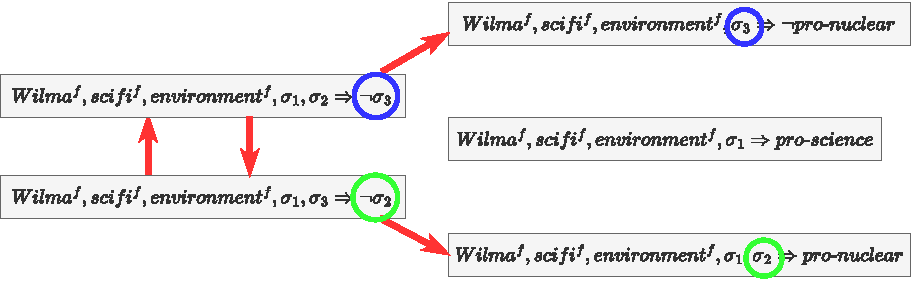
\includegraphics[scale=0.9]{pic/attack graph.pdf}
	\end{figure}
\end{frame}
    


\begin{frame}{Argumentation graph of Input/Output Logic Paradigm}
    \begin{figure}
		\centering
		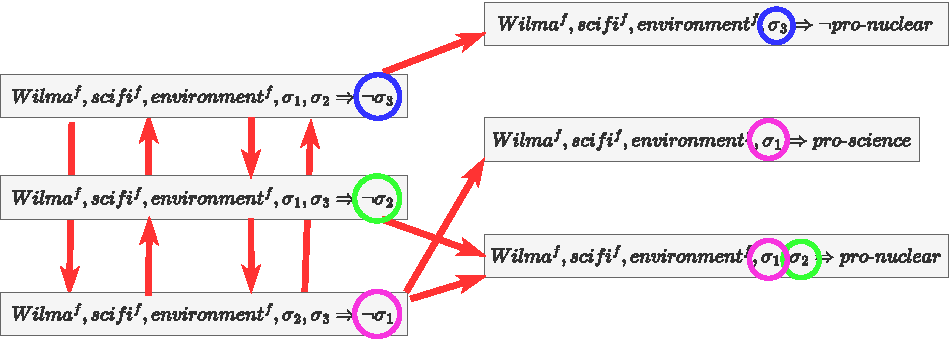
\includegraphics[scale=0.9]{pic/attack graph2.pdf}
	\end{figure}
\end{frame}
\end{comment}

\begin{frame}[label={sec:orgd9716e2},standout]{}
Let's sum up our 4 steps!
\end{frame}

\begin{frame}[label={sec:org9d76563}]{}
1. ~~ Given a knowledge base \(\mathbb{K} = \langle \mathcal{F}, \mathcal{D}, \mathcal{N} \rangle\) we let \alert{\(\mathsf{Args}(\mathbb{K})\)} be all sequents derivable in DAC whose left-hand-side is contained in \(\mathbb{K}\).
\pause

2. ~~ We define \alert{attacks} as expected: an argument attacks another one if the attackers conclusion expresses that some or all of the attacked argument's defaults / norms are not applicable.
\pause

3. ~~ We then apply \alert{argumentation semantics}. E.g., sets of arguments \(\mathcal{A}\) are to be
\begin{itemize}
\item conflict-free
\item stable (every argument not in \(\mathcal{A}\) is attacked by \(\mathcal{A}\) and \(\mathcal{A}\) is conflict-free),
\item etc.
\end{itemize}
\pause

4. ~~ On this basis, we define nonmonotonic \alert{consequence relations}.

\end{frame}

\begin{frame}[label={sec:org09f854e}]{Results}
\begin{itemize}
\item DAC with Def2 and without OR: every stable sets corresponds to a \alert{Reiter Default} extension and vice versa. \(\nc_1\) is Reiter's sceptical consequence. \pause
\item DAC with Def1: all 8 standard variants of (constrained) \alert{input-output logic} can be characterized analogously. \pause
\item We obtain a natural variant for \alert{default logic} with disjunction (see below). \pause
\item We obtain \alert{cautious variants} of default logic and IO-logic when opting for grounded argumentation semantics. \pause
\item The result is \alert{unifying}: only a minor twist in the proof-theory (Def1 vs Def2) leads to a Gestalt-switch in representation.
\end{itemize}
\end{frame}

\begin{comment}


\begin{frame}[label={sec:org035d8f2}]{Conjecture: Disjunctive Default Logic}
\begin{columns}
\begin{column}{.43\columnwidth}
Reiter:
\begin{bbox}
\begin{itemize}
\item Let \(\mathcal{O}_\star = \mathcal{F}\).
\item Loop:
\begin{itemize}
\item pick a default \(\delta = (\phi,\psi) \in \mathcal{D}\) for which \\[0pt]
(i, trigger) \(\mathcal{O}_\star \vdash \phi\), \\[0pt]
(ii, relevance) \(\psi \notin \mathcal{O}_{\star}\) and \\[0pt]
(iii, consistency) \(\mathcal{O}_{\star} \nvdash \neg\psi\)
\item let \(\mathcal{O}_{\star} = \mathcal{O}_{\star} \cup \{ \psi \}\)
\end{itemize}
\end{itemize}
\end{bbox}

\pause
\end{column}
\begin{column}{.57\columnwidth}
Our disjunctive variant:

\begin{bbox}
\begin{itemize}
\item Let \(\mathcal{O}_\star = \mathcal{F}\).
\item Loop:
\begin{itemize}
\item pick a \alert{family} of defaults \(\alert{\langle(\phi_i,\psi_i) \rangle_{i=1}^{m}} \subseteq \mathcal{D}\) for which \\[0pt]
(i, trigger) \(\mathcal{O}_\star \vdash \alert{\bigvee_{i=1}^m \phi_i}\), \\[0pt]
(ii, relevance) \(\alert{\bigvee_{i=1}^m \psi_i} \notin \mathcal{O}_{\star}\) and \\[0pt]
(iii, consistency) \(\mathcal{O}_\star \nvdash \neg \alert{\bigvee_{i=1}^m \psi_i}\)
\item let \(\mathcal{O}_{\star} = \mathcal{O}_{\star} \cup \{ \alert{\bigvee_{i=1}^m \psi_i} \}\)
\end{itemize}
\end{itemize}
\end{bbox}
\end{column}
\end{columns}
\end{frame}
\end{comment}


\section{Disjunctive Reasoning}
\label{sec:orgd76d5a1}

\begin{frame}[label={sec:orgb710fd7},standout]{More on disjunctions and hypothetical reasoning}
More on disjunctions and hypothetical reasoning \ldots{}

\vspace{2cm}

\emph{Joint work with \alert{Kees van Berkel}. Lots of inspiration from previous collaboration with \alert{Mathieu Beirlaen} and \alert{Jesse Heyninck} (see NMR 2018).}
\end{frame}

\begin{frame}{Example}
    Suppose our research group typically has for lunch burgers or pizza.  \pause

    When having burgers, we typically go to McBurger. {\it (But if that one is closed, there are other options for burgers ...)} \pause

    When having pizza, we typically go to Luigi's. \pause

    McBurger and Luigi's allow for cash payment. \pause

    On Mondays, McBurgers is typically closed. \pause 

    Today is Monday and we're about to have lunch.
\end{frame}

\begin{frame}[label={sec:org840feb7}]{Similarly}
\begin{tikzpicture}[scale=1, every node/.style={scale=1, align=center}, rounded corners, decorate, node distance = .3cm and 1.8cm]

\node [] (v) {\( \vee \)};
\node [ndnode, above = of v] (burger) {{\sf burger}};
\node [ndnode, below = of v] (pizza) {{\sf pizza}};

\begin{scope}[on background layer]
  \node [dnode, fit={(burger) (v) (pizza)}] (vee) {};
\end{scope}

\node [dnode, left = of vee] (lunch) {\sf Lunch};

\node [above = of vee, dnode] (Monday) {\sf Monday};

\node [ndnode, right = of burger] (mc) {{\sf McBurger}};
\node [ndnode, right = of pizza] (luigi) {{\sf Luigi}};
\node [ndnode, below right = of mc] (cash) {{\sf cash}};

\draw[darr] (lunch) to (vee);
\draw[darr] (burger) to (mc);
\draw[darr] (pizza) to (luigi);
\draw[darr] (mc.0) to [bend left] (cash);
\draw[darr] (luigi.0) to [bend right] (cash);

\draw[darr] (Monday.0) to [bend left] node [sloped] {\( \mid \)} (mc);

\draw[visible on = <2>, darr, draw=red] (vee) to (cash);
\end{tikzpicture}  

\pause

\[
\axs{\mathsf{burger} \Rightarrow \mathsf{McBurger}}
\axs{\mathsf{McBurger} \Rightarrow \mathsf{cash}}
\irl2{Cut}{\mathsf{burger} \Rightarrow \mathsf{cash}}
\axs{\mathsf{pizza} \Rightarrow \mathsf{Luigi}}
\axs{\mathsf{Luigi} \Rightarrow \mathsf{cash}}
\irl2{Cut}{\mathsf{pizza} \Rightarrow \mathsf{cash}}
\irl2{OR}{\alert{(\mathsf{burger} \vee \mathsf{pizza}) \Rightarrow \mathsf{cash}}}
\DP
\]
\end{frame}

\begin{frame}{Solution 1}
    The OR rule overgeneralizes, Gelfond \& Lifschitz's approach is not sufficiently fine-grained. What to do? \pause

Disjunctive Detachment:
    \begin{align*}
     \infer[\bf DisDet]{(\bigvee_{i=1}^n\alert{\phi_i})^{f}, \langle (\alert{\phi_{i}}, {\color{blue}\psi_i})^d \rangle_{i=1}^n \Rightarrow (\bigvee_{i=1}^n {\color{blue}\psi_i})^o} {\vphantom{M}}
     \end{align*}
\pause 

     Disjunctive Defeat:
     \begin{align*}
     \infer[\bf DisDef]{(\bigvee_{i=1}^n \phi_i)^f, \langle (\phi_{i}, \psi_i) \rangle_{i=2}^n, \alert{\neg\psi_1}^b \Rightarrow \neg(\phi_1, \alert{\psi_1})^d}{\vphantom{M}}
    \end{align*}
\end{frame}

\begin{frame}{In the example}

\def\d{\delta} \def\Lunch{{\sf lunch}}
\def\burger{{\sf burger}} \def\pizza{{\sf pizza}} \def\mc{{\sf McBurger}}
\def\cash{{\sf cash}}
\def\Monday{{\sf Monday}}

\scalebox{.8}{
    \begin{tikzpicture}[scale=1, every node/.style={scale=1, align=center}, rounded corners, decorate, node distance = .3cm and 1.8cm]

\node [] (v) {\( \vee \)};
\node [ndnode, above = of v] (burger) {{\sf burger}};
\node [ndnode, below = of v] (pizza) {{\sf pizza}};

\begin{scope}[on background layer]
  \node [dnode, fit={(burger) (v) (pizza)}] (vee) {};
\end{scope}

\node [dnode, left = of vee] (lunch) {\sf Lunch};

\node [above = of vee, dnode] (Monday) {\sf Monday};

\node [ndnode, right = of burger] (mc) {{\sf McBurger}};
\node [ndnode, right = of pizza] (luigi) {{\sf Luigi}};
\node [ndnode, below right = of mc] (cash) {{\sf cash}};

\draw[purple,darr] (lunch) to node[above]{$\d_1$} (vee);
\draw[purple,darr] (burger) to node[above]{$\d_2$} (mc);
\draw[purple,darr] (pizza) to node[above]{$\d_3$} (luigi);
\draw[purple,darr] (mc.0) to node[above]{$\d_4$} (cash);
\draw[purple,darr] (luigi.0) to node[above]{$\d_5$} (cash);

\draw[darr] (Monday.0) to [bend left] node[above]{$\d_6$} node [sloped] {\( {\mid} \)} (mc);
\end{tikzpicture}  
}

\medskip
\def\d{\delta} \def\Lunch{{\sf lunch}}
\def\burger{{\sf bur}} \def\pizza{{\sf piz}} \def\mc{{\sf McB}}
\def\cash{{\sf cash}}
\def\Monday{{\sf Mon}}

\scalebox{.9}{
    \[
    \axs{}
    \irr1{DisDet}{\seqq{(\mc \vee {\sf Lui})^b, \d_4, \d_5}{\cash^b}}
    \axs{}
    \irr1{DisDet}{\seqq{(\burger \vee \pizza)^b, \d_2, \d_3}{(\mc \vee {\sf Lui})^b}}
    \irl2{}{\seqq{(\burger \vee \pizza)^b, \d_2, \d_3, \d_4, \d_5}{\cash^b}}
    \axs{\seqq{\Lunch^f, \d_1}{(\burger \vee \pizza)^b}}
    \irl2{}{\seqq{\Lunch^f, \d_1,\ldots,\d_5}{\cash^b}}
    \DP
    \]
}
    
\end{frame}

\begin{frame}{In the example}
    \def\d{\delta} \def\Lunch{{\sf lunch}}
\def\burger{{\sf burger}} \def\pizza{{\sf pizza}} \def\mc{{\sf McBurger}}
\def\cash{{\sf cash}}
\def\Monday{{\sf Monday}}

\scalebox{.8}{
    \begin{tikzpicture}[scale=1, every node/.style={scale=1, align=center}, rounded corners, decorate, node distance = .3cm and 1.8cm]

\node [] (v) {\( \vee \)};
\node [ndnode, above = of v] (burger) {{\sf burger}};
\node [ndnode, below = of v] (pizza) {{\sf pizza}};

\begin{scope}[on background layer]
  \node [dnode, fit={(burger) (v) (pizza)}] (vee) {};
\end{scope}

\node [dnode, left = of vee] (lunch) {\sf Lunch};

\node [above = of vee, dnode] (Monday) {\sf Monday};

\node [ndnode, right = of burger] (mc) {{\sf McBurger}};
\node [ndnode, right = of pizza] (luigi) {{\sf Luigi}};
\node [ndnode, below right = of mc] (cash) {{\sf cash}};

\draw[purple,darr] (lunch) to node[above]{$\d_1$} (vee);
\draw[darr] (burger) to node[above]{$\d_2$} (mc);
\draw[purple,darr] (pizza) to node[above]{$\d_3$} (luigi);
\draw[darr] (mc.0) to node[above]{$\d_4$} (cash);
\draw[darr] (luigi.0) to node[above]{$\d_5$} (cash);

\draw[purple,darr] (Monday.0) to [bend left] node[above]{$\d_6$} node [sloped] {\( {\mid} \)} (mc);
\end{tikzpicture}  
}
\medskip

\def\d{\delta} \def\Lunch{{\sf lunch}}
\def\burger{{\sf bur}} \def\pizza{{\sf piz}} \def\mc{{\sf McB}}
\def\cash{{\sf cash}}
\def\Monday{{\sf Mon}}

\scalebox{.9}{
    \[
    \axs{}
    \irr1{DisDef}{\seqq{(\burger \vee \pizza)^b, \neg \mc^b, \d_3}{\neg \d_2}}
    \axs{\seqq{\Monday^f, \d_6}{\neg \mc^b}}
    \irr2{Cut}{\seqq{\Monday^f, (\burger\vee\pizza)^b, \d_3, \d_6}{\neg \d_2}}
    \axs{\seqq{\Lunch^f, \d_1}{(\burger \vee \pizza)^b}}
    \irl2{Cut}{\seqq{\Lunch^f, \Monday^f, \d_1, \d_3, \d_6}{\neg\d_2}}
    \DP
    \]
}
    
\end{frame}

\begin{frame}{In the example}
\def\d{\delta} \def\Lunch{{\sf lunch}}
\def\burger{{\sf burger}} \def\pizza{{\sf pizza}} \def\mc{{\sf McBurger}}
\def\cash{{\sf cash}}
\def\Monday{{\sf Monday}}

    \begin{tikzpicture}[scale=1, every node/.style={scale=1, align=center}, rounded corners, decorate, node distance = .1cm and 1.8cm]

\node [] (v) {\( \vee \)};
\node [ndnode, above = of v] (burger) {{\sf burger}};
\node [ndnode, below = of v] (pizza) {{\sf pizza}};

\begin{scope}[on background layer]
  \node [dnode, fit={(burger) (v) (pizza)}] (vee) {};
\end{scope}

\node [dnode, left = of vee] (lunch) {\sf Lunch};

\node [above = of vee, dnode] (Monday) {\sf Monday};

\node [ndnode, right = of burger] (mc) {{\sf McBurger}};
\node [ndnode, right = of pizza] (luigi) {{\sf Luigi}};
\node [ndnode, below right = of mc] (cash) {{\sf cash}};

\draw[darr] (lunch) to node[above]{$\d_1$} (vee);
\draw[darr] (burger) to node[above]{$\d_2$} (mc);
\draw[darr] (pizza) to node[above]{$\d_3$} (luigi);
\draw[darr] (mc.0) to node[above]{$\d_4$} (cash);
\draw[darr] (luigi.0) to node[above]{$\d_5$} (cash);

\draw[darr] (Monday.0) to [bend left] node[above]{$\d_6$} node [sloped] {\( \boldsymbol{\mid} \)} (mc);
\end{tikzpicture}  

\medskip

    \begin{tikzpicture}[every node/.style={ospale}, node distance = .5cm and .5cm]
    \node [os] (a) {\afnodeflat{a}{\Lunch^f,\d_1}{(\burger\vee \pizza)^b}};
    \node [right = of a] (b) {\afnodeflat{b}{\Lunch^f,\d_1,\d_2,\d_3,\d_4,\d_5}{\cash^b}};
    \node [os, below = of a] (c) {\afnodeflat{c}{\Monday^f,\d_6}{\neg \mc}};
    \node [os, right = of c] (d) {\afnodeflat{d}{\Lunch^f, \Monday^f, \d_1, \d_6}{\neg \d_2}};

    \draw[att,->] (d) to (b);
    
    \end{tikzpicture}
\end{frame}

\begin{frame}{Disjunctive Default Logic}
    In a forthcoming paper we define a version of Reiter's greedy algorithm and show that every default extension corresponds to a stable set and vice versa.

    [ask for details!]
\end{frame}

\begin{frame}[standout]{}
    But, we're not happy, yet!
\end{frame}

\begin{frame}[label={sec:org9143424}]{More trouble with disjunctions}
\begin{tikzpicture}[scale=1, every node/.style={scale=1, align=center}, rounded corners, decorate, node distance = .3cm and 1.8cm]
\node [dnode] (Anne) {\sf Anne};
\node [dnode, right = of Anne] (rat) {\sf Rationalist};
\node [ndnode, above right = of rat] (sci) {\sf pro-science};

\node [ndnode, below right = of rat] (env)   {\sf environmentalist};
\node [ndnode, right = of sci] (progmo) {\sf pro-gmo};
\node [ndnode, right = of env] (cgmo) {\sf \( \neg \)pro-gmo};

\draw[sarr] (Anne) to (rat);
\draw[darr] (rat) to [bend left] (sci.180);
\draw[darr] (rat) to [bend right] (env.180);
\draw[darr] (sci) to (progmo);
\draw[darr] (env.0) to (cgmo);
\end{tikzpicture}  
\pause 
Here we should stay \alert{agnostic} about \textsf{pro-gmo}.
\end{frame}


\begin{frame}[label={sec:org5ae42de},fragile]{Problematic Example}
\begin{tikzpicture}[scale=1, every node/.style={scale=1, align=center}, rounded corners, decorate, node distance = .3cm and 1.8cm]
\node [dnode] (Anne) {\( a \): {\sf Anne}};

\node [right = of Anne] (v) {\( \vee \)};
\node [ndnode, above = of v] (rat) {\( r \): {\sf Rationalist}};
\node [ndnode, below = of v] (cre) {\( c \): {\sf creationist}};

\begin{scope}[on background layer]
  \node [dnode, fit={(rat) (v) (cre)}] (vee) {};
\end{scope}

\node [ndnode, above right = of rat] (sci) {\( s \): {\sf pro-science}};

\node [ndnode, below right = of rat] (env)   {\( e \) : {\sf environmentalist}};
\node [ndnode, right = of sci] (progmo) {\( g \): {\sf pro-gmo}};
\node [ndnode, right = of env] (cgmo) {\( \neg g \) : {\sf \( \neg \)pro-gmo}};

\draw[sarr] (Anne) to (vee);
\draw[darr] (rat) to (sci.180);
\draw[darr] (rat) to (env.180);
\draw[darr] (sci) to (progmo);
\draw[darr] (env.0) to (cgmo);
\draw[darr] (cre.0) to [bend right] (cgmo);

\draw[visible on=<2>, darr, draw=red] (vee.0) to [bend right] (cgmo.190);
\end{tikzpicture}  

\pause
With the OR rule:

\[
\axs{r \Rightarrow e}
\axs{e \Rightarrow \neg g}
\irl2{Cut}{r \Rightarrow \neg g}
\axs{c \Rightarrow \neg g}
\irl2{OR}{\alert{(r \vee c) \Rightarrow \neg g}}
\DP
\]
\end{frame}

\begin{frame}{Similarly with our first solution}
\def\d{\delta}
    \begin{tikzpicture}[scale=1, every node/.style={scale=1, align=center}, rounded corners, decorate, node distance = .3cm and 1.8cm]
\node [dnode] (Anne) {\( a \): {\sf Anne}};

\node [right = of Anne] (v) {\( \vee \)};
\node [ndnode, above = of v] (rat) {\( r \): {\sf Rationalist}};
\node [ndnode, below = of v] (cre) {\( c \): {\sf creationist}};

\begin{scope}[on background layer]
  \node [dnode, fit={(rat) (v) (cre)}] (vee) {};
\end{scope}

\node [ndnode, above right = of rat] (sci) {\( s \): {\sf pro-science}};

\node [ndnode, below right = of rat] (env)   {\( e \) : {\sf environmentalist}};
\node [ndnode, right = of sci] (progmo) {\( g \): {\sf pro-gmo}};
\node [ndnode, right = of env] (cgmo) {\( \neg g \) : {\sf \( \neg \)pro-gmo}};

\draw[purple,sarr] (Anne) to node[above]{$\sigma$} (vee);
\draw[darr] (rat) to node[above]{$\d_1$} (sci.180);
\draw[purple,darr] (rat) to node[above]{$\d_2$} (env.180);
\draw[darr] (sci) to node[above]{$\d_3$} (progmo);
\draw[purple,darr] (env.0) to node[above]{$\d_4$} (cgmo);
\draw[purple,darr] (cre.0) to [bend right] node[above] {$\d_5$} (cgmo);
\end{tikzpicture}  

We get the argument
\[
{\sf Anna}^f, \sigma, \d_2, \d_4, \d_5 \Rightarrow \neg {\sf pro\mbox{-}gmo}^b
\]
but we don't have a counter-argument!
\end{frame}


\begin{frame}[label={sec:org6b86e0c}]{Solution 2 (work in progress)}
We need to track our assumptions when reasoning with cases!

Inspiration: natural deduction.

\vspace{-.5cm}

\[
\axs{\array{c} \phantom{M} \\ \phantom{M} \\ \phi \vee \psi \endarray}
\axs{\mbox{hyp.~arg.~1} \left\{ \array{c} \phi \\ \vdots \\ \gamma \endarray \right.}
\axs{\left. \array{c} \psi \\ \vdots \\ \gamma \endarray \right\} \mbox{hyp.~arg.~2} }
\irl3{RbC}{\gamma}
\DP
\]

\pause

\[
\axs{\array{c} \phantom{M} \\ \phantom{M} \\ \phantom{M} \\ \phantom{M} \\ \phi \vee \psi \endarray}
\axs{\substack{\mbox{hyp.~arg.~1} \\ \mbox{\it possible} \\ \mbox{\it defeat}} \left\{ \array{c} \phi \\ \Downarrow \\ \vdots \\ \Downarrow \\ \gamma \endarray \right.}
\axs{\left. \array{c} \psi \\ \Downarrow \\ \vdots \\ \Downarrow \\ \gamma \endarray \right\} \substack{\mbox{hyp.~arg.~2} \\ \mbox{\it possible} \\ \mbox{\it defeat}} }
\irl3{RbC}{\gamma}
\DP
\]
\end{frame}
\begin{frame}[label={sec:org0c5900f}]{A solution (work in progress)}
\[
\axs{\array{c} \phantom{M} \\ \phantom{M} \\ \phantom{M} \\ \phantom{M} \\ \mathsf{pizza} \vee \mathsf{burger} \endarray}
\axs{\array{c} \mathsf{pizza} \\ \Downarrow \\ \mathsf{Luigi} \\ \Downarrow \\ \mathsf{cash} \endarray}
\axs{\array{l} \mathsf{burger} \\ ~~~~\Downarrow \\ \alert{\mathsf{McBurger}} \quad \not\Leftarrow \mathsf{Monday} \\ ~~~\Downarrow \\ \mathsf{cash} \endarray}
\irl3{RbC}{\mathsf{cash}}
\DP
\]
\end{frame}

\begin{frame}[label={sec:orga73835f}]{Enhancing DAC with Hypothetical Arguments: HDAC}
\[
\axs{s_1: \phi_1^{\alert{h}}, \Gamma_1 \Rightarrow_{\alert{\Theta_1}} \psi}
\axs{s_2: \phi_2^{\alert{h}}, \Gamma_2 \Rightarrow_{\alert{\Theta_2}} \psi}
\irl2{HOR}{(\phi_1 \vee \phi_2)^{\alert{h}}, \Gamma_1, \Gamma_2 \Rightarrow_{\alert{s_1, s_2, \Theta_1, \Theta_2}} \psi}
\DP
\]
\pause
\vspace{.5cm}
\[
\axs{\phi^f, \Gamma \Rightarrow_{\Theta} \Delta}
\irl1{HDet1}{\phi^{\alert{h}}, \Gamma \Rightarrow_{\Theta} \Delta}
\DP 
\]

\[
\axs{\phi^{\alert{h}}, \Gamma \Rightarrow_{\Theta} \Delta}
\irl1{HDet2}{\phi^{b/o}, \Gamma \Rightarrow_{\Theta} \Delta}
\DP
\]
\end{frame}

\begin{frame}[label={sec:org27bba33}]{}
\begin{tikzpicture}[scale=.8, every node/.style={scale=.8, align=center}, rounded corners, decorate, node distance = .3cm and 1.8cm]

\node [] (v) {\( \vee \)};
\node [ndnode, above = of v] (burger) {{\sf burger}};
\node [ndnode, below = of v] (pizza) {{\sf pizza}};

\begin{scope}[on background layer]
  \node [ndnode, fit={(burger) (v) (pizza)}] (vee) {};
\end{scope}

\node [dnode, left = of vee] (lunch) {\sf Lunch};

\node [above = of vee, dnode] (Monday) {\sf Monday};

\node [ndnode, right = of burger] (mc) {{\sf McBurger}};
\node [ndnode, right = of pizza] (luigi) {{\sf Luigi}};
\node [ndnode, below right = of mc] (cash) {{\sf cash}};

\draw[darr] (lunch) to node[above] {\( \delta_1 \)} (vee);
\draw[darr] (burger) to node[above] {\( \delta_2 \)} (mc);
\draw[darr] (pizza) to node[above] {\( \delta_3 \)} (luigi);
\draw[darr] (mc.0) to [bend left] node[above] {\( \delta_4 \)} (cash);
\draw[darr] (luigi.0) to [bend right] node[above] {\( \delta_5 \)} (cash);

\draw[darr] (Monday.0) to [bend left] node[above,pos=.4] {\( \delta_6 \)} node [sloped] {\( \mid \)} (mc);
\end{tikzpicture}  


\[
\axs{\mathsf{burger}^f, \delta_2, \delta_4 \Rightarrow_{\emptyset}\mathsf{cash}^b}
\irl1{HDet1}{s_1: \mathsf{burger}^h, \delta_2, \delta_4 \Rightarrow_{\emptyset} \mathsf{cash}^b}
\axs{\mathsf{pizza}^f, \delta_3, \delta_5 \Rightarrow_{\emptyset} \mathsf{cash}^b}
\irl1{HDet1}{s_2: \mathsf{pizza}^h, \delta_3, \delta_5 \Rightarrow_{\emptyset} \mathsf{cash}^b}
\irl2{HOR}{(\mathsf{burger} \vee \mathsf{pizza})^h, \delta_2, \delta_4 \Rightarrow_{s_1, s_2} \mathsf{cash}^b}
\irl1{HDet2}{\array{c}(\mathsf{burger} \vee \mathsf{pizza})^b, \delta_2, \delta_4 \Rightarrow_{s_1, s_2} \mathsf{cash}^b \\ \vdots \endarray}
\irl1{}{\mathsf{Lunch}^{f}, \delta_1, \dotsc, \delta_5 \Rightarrow_{s_{1},s_2} \mathsf{cash}^b}
\DP
\]
\end{frame}
\def\Hyp{\mathsf{Hyp}}
\begin{frame}{Attacks and Defeats}
    We define undercut attacks as before: 
    \begin{center}$\Gamma \Rightarrow_\Omega \neg(\phi,\psi)$ \alert{attacks} $\Delta, (\phi,\psi) \Rightarrow_{\Lambda} \sigma$.
    \end{center}
    \pause

    But now all attacks are successful. In particular, attacks by arguments that contain hypothetical assumptions that are not contained in the attacked argument fail. Successful attacks are called \alert{defeats}. 
    \pause
    
    We let \alert{$\Hyp(\Gamma \Rightarrow_\Omega \psi)$} be the set of $h$-labeled formulas in $\Gamma$.

    For instance, $\Hyp(\alert{\mathsf{burger}^h}, \delta_2, \delta_4 \Rightarrow_\emptyset \mathsf{cash}^b) = \{ \alert{\mathsf{burger}} \}$.

    \pause

    Then, 
    \begin{center} ${\color{blue}s} : \Gamma \Rightarrow_\Omega \neg(\phi,\psi)$ \alert{defeats} ${\color{red}t} : \Delta, (\phi,\psi) \Rightarrow_\Lambda \sigma$, ~~ if $\Hyp({\color{blue}s}) 
    \subseteq \Hyp({\color{red}t})$. \\ \pause
    ${\color{blue}s} : \Gamma \Rightarrow_\Omega \neg(\phi,\psi)$ \alert{defeats} ${\color{red} t}: \Delta \Rightarrow_{\color{purple}\Lambda} \sigma$, ~~ if it defeats some $t' \in {\color{purple}\Lambda}$.
    \end{center}
\end{frame}

\begin{comment}
\begin{frame}[label={sec:org013357e},fragile]{Argumentation with Hypothetical Arguments}
	 Let $\mathsf{Sub}(t)$ for the sequents set in the subscript of $t$, and  $$\mathsf{Hyp}^*(s)=\{\phi^h\mid \phi^h\in\Omega^h\cap \mathsf{formula}(s)\},$$
	$$\mathsf{Hyp}(s)=\mathsf{Hyp}^*(s)\cup \bigcup\{\mathsf{Hyp}^*(t)\mid s\in \mathsf{Sub}(t)\}.$$
	\pause
	We not only consider all \textit{h-assumptions} of $s$, but also all \textit{h-assumptions} of those arguments containing $s$.
\end{frame}
\end{comment}

\begin{frame}{}
    \def\lunch{\mathsf{lunch}} \def\d{\delta} \def\Monday{\mathsf{Monday}}
    \def\burger{\mathsf{burger}} \def\pizza{\mathsf{pizza}} \def\cash{\mathsf{cash}}
    \def\McBurger{\mathsf{McBurger}}
    
    \begin{tikzpicture}[scale=.7, every node/.style={ospale, scale=.8}, node distance=.6cm and .5cm]
        \node [os] (a) {\afnodeflat{a}{\lunch^f,\d_1}{(\burger\vee\pizza)^b}};
        \node [right = of a] (h2) {\afnodeflat{h_2}{\Monday^f,\burger^h,\d_2}{\neg\d_6}};
        \node [os, below = of a] (b1) {\afnodeflat{b_1}{\Monday^f,\d_6}{\McBurger^b}};
        \node [below = of b1] (g) {\afnodeflat{g}{\pizza^h,\d_3,\d_5}{\cash^b}};
        \node [os, right = of b1] (b2) {\afnodeflat{h_3}{\Monday^f,\burger^h,\d_6}{\neg\d_2}};
        \node [right = of b2] (h1) {\afnodeflat{h_1}{\burger^h,\d_2,\d_4}{\cash^b}};
        \node [below = of b2] (c) {\afnodeH{c}{\lunch^f,\d_1,\d_2,\d_3,\d_4,\d_5}{h_1,g}{\cash^b}};

        \draw[att,<->] (b2) to (h2);
        \draw[att,->] (b2) to (c);
        \draw[att,->] (b2) to (h1);
        \draw[att,->, dotted] (h2) to (b1); 
    \end{tikzpicture}

    \medskip

    \begin{tikzpicture}[scale=.8, every node/.style={scale=.8, align=center}, rounded corners, decorate, node distance = .3cm and 1.8cm]
\node [] (v) {\( \vee \)};
\node [ndnode, above = of v] (burger) {{\sf burger}};
\node [ndnode, below = of v] (pizza) {{\sf pizza}};
\begin{scope}[on background layer]
  \node [dnode, fit={(burger) (v) (pizza)}] (vee) {};
\end{scope}
\node [dnode, left = of vee] (lunch) {\sf Lunch};
\node [above = of vee, dnode] (Monday) {\sf Monday};
\node [dnode, right = of burger] (mc) {{\sf McBurger}};
\node [ndnode, right = of pizza] (luigi) {{\sf Luigi}};
\node [ndnode, below right = of mc] (cash) {{\sf cash}};
\draw[purple,darr] (lunch) to node[above] {\( \delta_1 \)} (vee);
\draw[darr] (burger) to node[above] {\( \delta_2 \)} (mc);
\draw[darr] (pizza) to node[above] {\( \delta_3 \)} (luigi);
\draw[darr] (mc.0) to [bend left] node[above] {\( \delta_4 \)} (cash);
\draw[darr] (luigi.0) to [bend right] node[above] {\( \delta_5 \)} (cash);
\draw[purple,darr] (Monday.0) to [bend left] node[above,pos=.4] {\( \delta_6 \)} node [sloped] {\( \mid \)} (mc);
\end{tikzpicture}  
\end{frame}

% C: It would be interesting to work here with a prioritized disjunction (Brewka?!): 
% burger => McBurger | KingBurger 
% burger => cash
% KingBurger => \neg cash

\begin{frame}{Back to our problematic example for Solution 1}
    \def\d{\delta} \def\Anne{\mathsf{An}}
    \begin{tikzpicture}[scale=1, every node/.style={scale=1, align=center}, rounded corners, decorate, node distance = .1cm and 1.8cm]
\node [dnode] (Anne) {\( \Anne \): {\sf Anne}};

\node [right = of Anne] (v) {\( \vee \)};
\node [ndnode, above = of v] (rat) {\( r \): {\sf Rationalist}};
\node [ndnode, below = of v] (cre) {\( c \): {\sf creationist}};

\begin{scope}[on background layer]
  \node [dnode, fit={(rat) (v) (cre)}] (vee) {};
\end{scope}

\node [ndnode, above right = of rat] (sci) {\( s \): {\sf pro-science}};

\node [ndnode, below right = of rat] (env)   {\( e \) : {\sf environmentalist}};
\node [ndnode, right = of sci] (progmo) {\( g \): {\sf pro-gmo}};
\node [ndnode, right = of env] (cgmo) {\( \neg g \) : {\sf \( \neg \)pro-gmo}};

\draw[sarr] (Anne) to node[above]{$\sigma$} (vee);
\draw[darr] (rat) to node[above]{$\d_1$} (sci.180);
\draw[darr] (rat) to node[above]{$\d_2$} (env.180);
\draw[darr] (sci) to node[above]{$\d_3$} (progmo);
\draw[darr] (env.0) to node[above]{$\d_4$} (cgmo);
\draw[darr] (cre.0) to [bend right] node[above] {$\d_5$} (cgmo);
\end{tikzpicture}  

\begin{tikzpicture}[every node/.style={ospale}, node distance = .4cm and .5cm]
    \node (a) {\afnodeH{a}{\Anne^f, \sigma, \d_2, \d_4, \d_5}{h_1,h_2}{\neg g^b}};
    \node [right = of a] (h1) {\afnodeH{h_1}{r^h, \d_2, \d_4}{\emptyset}{\neg g^b}};
    \node [os, below = of h1] (h3) {\afnodeH{h_3}{r^h, \d_1, \d_2, \d_3}{\emptyset}{\neg \d_4}};
    \node [os, left = of a] (h2) {\afnodeH{h_2}{c^h, \d5}{\emptyset}{\neg g}};
    \node [below = of a] (h4) {\afnodeH{h_4}{r^h, \d_1, \d_2, \d_4}{\emptyset}{\neg \d_3}};
    \node [os, below = of h2] (b) {\afnodeH{b}{\Anne^f, \sigma}{\emptyset}{(r \vee c)^b}};

    \draw[att,<->] (h3) to (h4);
    \draw[att,->] (h3) to (a);
    \draw[att,->] (h3) to (h1);
    
\end{tikzpicture}
\end{frame}

\begin{frame}{Back to our problematic example for Solution 1}
    \def\d{\delta} \def\Anne{\mathsf{An}}
    \begin{tikzpicture}[scale=1, every node/.style={scale=1, align=center}, rounded corners, decorate, node distance = .1cm and 1.8cm]
\node [dnode] (Anne) {\( \Anne \): {\sf Anne}};

\node [right = of Anne] (v) {\( \vee \)};
\node [ndnode, above = of v] (rat) {\( r \): {\sf Rationalist}};
\node [ndnode, below = of v] (cre) {\( c \): {\sf creationist}};

\begin{scope}[on background layer]
  \node [dnode, fit={(rat) (v) (cre)}] (vee) {};
\end{scope}

\node [ndnode, above right = of rat] (sci) {\( s \): {\sf pro-science}};

\node [ndnode, below right = of rat] (env)   {\( e \) : {\sf environmentalist}};
\node [ndnode, right = of sci] (progmo) {\( g \): {\sf pro-gmo}};
\node [ndnode, right = of env] (cgmo) {\( \neg g \) : {\sf \( \neg \)pro-gmo}};

\draw[sarr] (Anne) to node[above]{$\sigma$} (vee);
\draw[darr] (rat) to node[above]{$\d_1$} (sci.180);
\draw[darr] (rat) to node[above]{$\d_2$} (env.180);
\draw[darr] (sci) to node[above]{$\d_3$} (progmo);
\draw[darr] (env.0) to node[above]{$\d_4$} (cgmo);
\draw[darr] (cre.0) to [bend right] node[above] {$\d_5$} (cgmo);
\end{tikzpicture}  

\begin{tikzpicture}[every node/.style={ospale}, node distance = .4cm and .5cm]
    \node [os] (a) {\afnodeH{a}{\Anne^f, \sigma, \d_2, \d_4, \d_5}{h_1,h_2}{\neg g^b}};
    \node [os, right = of a] (h1) {\afnodeH{h_1}{r^h, \d_2, \d_4}{\emptyset}{\neg g^b}};
    \node [below = of h1] (h3) {\afnodeH{h_3}{r^h, \d_1, \d_2, \d_3}{\emptyset}{\neg \d_4}};
    \node [os, left = of a] (h2) {\afnodeH{h_2}{c^h, \d5}{\emptyset}{\neg g}};
    \node [os, below = of a] (h4) {\afnodeH{h_4}{r^h, \d_1, \d_2, \d_4}{\emptyset}{\neg \d_3}};
    \node [os, below = of h2] (b) {\afnodeH{b}{\Anne^f, \sigma}{\emptyset}{(r \vee c)^b}};

    \draw[att,<->] (h3) to (h4);
    \draw[att,->] (h3) to (a);
    \draw[att,->] (h3) to (h1);
    
\end{tikzpicture}
\end{frame}

\begin{frame}{}
    Compared to DAC with OR we may loose consequences, such as $\neg \mathsf{pro\mbox{-}gmo}^b$ in this case. (But this is as desired!)

    \pause

    In some cases we may also gain consequences, for instance $v$ in:

\begin{center}
    \begin{tikzpicture}[scale=.8, every node/.style={scale=.8, align=center}, rounded corners, decorate, node distance = .3cm and 1.8cm]
\node [] (v) {\( \vee \)};
\node [ndnode, above = of v] (burger) {\( p \)};
\node [ndnode, below = of v] (pizza) {\( q \)};
\begin{scope}[on background layer]
  \node [dnode, fit={(burger) (v) (pizza)}] (vee) {};
\end{scope}
\node [dnode, left = of vee] (lunch) {$f_1$};
\node [above = 1.3cm of vee, dnode] (Monday) {$f_2$};
\node [dnode, right = of burger] (mc) {\( u \)};
\node [dnode, below right = of mc] (cash) {\( v \)};
\draw[purple,darr] (lunch) to node[above] {\( \delta_1 \)} (vee);
\draw[darr] (burger) to node[above] {\( \delta_2 \)} (mc);
\draw[darr] (pizza) to node[above] {\( \delta_3 \)} (cash);
\draw[darr] (mc.0) to node[above] {\( \delta_4 \)} node[sloped] {$\mid$} (cash);
\draw[purple,darr] (Monday.0) to [bend left] node[above,pos=.4] {\( \delta_6 \)} (cash);
\draw[purple,darr] (Monday) to node[above] {$\delta_5$}node[sloped] {$\mid$}  (mc);
\end{tikzpicture}
\end{center}

Is this as desired?
\end{frame}


\begin{frame}{Did we massage intuitions?}
    Suppose our research group typically has for lunch burgers or pizza. 

    When having burgers, we typically go to McBurger. {\it (But if that one is closed, there are other options for burgers ...)}

    \alert{If we go for burgers and McBurger is closed, we typically go to KingBurger. At KingBurger we typically pay with credit card.}

    When having pizza, we typically go to Luigi's.

    McBurger and Luigi's allow for cash payment.

    On Mondays, McBurgers is typically closed.

    Today is Monday and we're about to have lunch.
\end{frame}

\begin{frame}{DAC with OR}
     \begin{tikzpicture}[scale=.8, every node/.style={scale=.8, align=center}, rounded corners, decorate, node distance = .3cm and 1.8cm]
\node [] (v) {\( \vee \)};
\node [ndnode, above = of v] (burger) {{\sf burger}};
\node [ndnode, below = of v] (pizza) {{\sf pizza}};
\begin{scope}[on background layer]
  \node [dnode, fit={(burger) (v) (pizza)}] (vee) {};
\end{scope}
\node [dnode, left = of vee] (lunch) {\sf Lunch};
\node [above = 1.3cm of lunch, dnode] (Monday) {\sf Monday};
\node [above = 1.3cm of vee, dnode] (nMc) {$\neg$ {\sf McBurger}};
\draw[-] (burger) to node[ospale] (wedge) {$\wedge$} (nMc);
\node [ospale,right = of wedge] (king) {\sf KingBurger};
\draw[darr] (wedge) to node[above] {$\delta_2$} (king);
\node [ospale,right = of king] (ncash) {$\neg$ {\sf cash}};
\node [ndnode, right = of pizza] (luigi) {{\sf Luigi}};
\node [dnode, above right = of luigi] (cash) {{\sf cash}};
\node [ndnode, right = of burger] (mc) {\sf McBurger};
\draw[darr] (burger) to node[above] {$\delta_7$} (mc);
\draw[darr] (mc) to node[above] {$\delta_8$} (cash);
\draw[purple,darr] (lunch) to node[above] {\( \delta_1 \)} (vee);
\draw[darr] (pizza) to node[above] {\( \delta_3 \)} (luigi);
\draw[darr] (king) to node[above] {\( \delta_4 \)} (ncash);
\draw[darr] (luigi) to node[above] {\( \delta_5 \)} (cash);
\draw[purple,darr] (Monday) to node[above] {$\delta_6$} (nMc);
\draw[darr,red] (vee) to (cash);
\end{tikzpicture}

So, ${\sf cash}$ is a consequence.
\end{frame}

\begin{frame}{HDAC}
\begin{tikzpicture}[scale=.8, every node/.style={scale=.8, align=center}, rounded corners, decorate, node distance = .3cm and 1.8cm]
\node [] (v) {\( \vee \)};
\node [ndnode, above = of v] (burger) {{\sf burger}};
\node [ndnode, below = of v] (pizza) {{\sf pizza}};
\begin{scope}[on background layer]
  \node [dnode, fit={(burger) (v) (pizza)}] (vee) {};
\end{scope}
\node [dnode, left = of vee] (lunch) {\sf Lunch};
\node [above = 1.3cm of lunch, dnode] (Monday) {\sf Monday};
\node [above = 1.3cm of vee, dnode] (nMc) {$\neg$ {\sf McBurger}};
\draw[-] (burger) to node[ospale] (wedge) {$\wedge$} (nMc);
\node [ospale,right = of wedge] (king) {\sf KingBurger};
\draw[darr] (wedge) to node[above] {$\delta_2$} (king);
\node [ospale,right = of king] (ncash) {$\neg$ {\sf cash}};
\node [ndnode, right = of pizza] (luigi) {{\sf Luigi}};
\node [ndnode, above right = of luigi] (cash) {{\sf cash}};
\node [ndnode, right = of burger] (mc) {\sf McBurger};
\draw[darr] (burger) to node[above] {$\delta_7$} (mc);
\draw[darr] (mc) to node[above] {$\delta_8$} (cash);
\draw[green,darr] (lunch) to node[above] {\( \delta_1 \)} (vee);
\draw[darr] (pizza) to node[above] {\( \delta_3 \)} (luigi);
\draw[darr] (king) to node[above] {\( \delta_4 \)} (ncash);
\draw[darr] (luigi) to node[above] {\( \delta_5 \)} (cash);
\draw[darr] (Monday) to node[above] {$\delta_6$} (nMc);
% \draw[darr,red] (vee) to (cash);
\end{tikzpicture}

We get neither ${\sf cash}$ nor $\neg {\sf cash}$ as a consequence, as expected.
\end{frame}

\begin{frame}{Hypothetical consequences}
    $\mathbb{K} \nc_1 \alert{(\Pi \leadsto \psi)}$ ~~iff~~ in every stable set $\mathcal{A}$ there is an argument $a$ with $\Hyp(a) \subseteq \Pi$ with conclusion $\psi$. \hfill [similar for $\nc_2$]
    \pause

    In our example we have the following hypothetical consequences: 

    \medskip
    
    \begin{columns}
    \begin{column}{.35\textwidth}
    \begin{itemize}
        \item<3-> $\alert<3-4>{\sf pizza} \leadsto {\sf Luigi}$
        \item<4-> $\alert<4>{\sf pizza} \leadsto {\sf cash}$
        \item<5-> $\alert<5-6>{\sf burger} \leadsto {\sf KingBurger}$
        \item<6-> $\alert<6>{\sf burger} \leadsto \neg{\sf cash}$ 
    \end{itemize}
    \end{column}

\begin{column}{.65\textwidth}
\scalebox{1}{
    \begin{tikzpicture}[scale=.8, every node/.style={scale=.8, align=center}, rounded corners, decorate, node distance = .3cm and 1.4cm]
\node [] (v) {\( \vee \)};
\node [ndnode, above = of v] (burger) {\alert<5-6>{\sf burger}};
\node [ndnode, below = of v] (pizza) {\alert<3-4>{\sf pizza}};
\begin{scope}[on background layer]
  \node [dnode, fit={(burger) (v) (pizza)}] (vee) {};
\end{scope}
\node [dnode, left = of vee] (lunch) {\sf Lunch};
\node [above = 1.3cm of lunch, dnode] (Monday) {\sf Monday};
\node [above = 1.3cm of vee, dnode] (nMc) {$\neg$ {\sf McBurger}};
\draw[-] (burger) to node[ospale] (wedge) {$\wedge$} (nMc);
\node [ospale,right = of wedge] (king) {\alert<5-6>{\sf KingBurger}};
\draw[darr] (wedge) to node[above] {$\delta_2$} (king);
\node [ospale,right = of king] (ncash) {\alert<4>{\alert<6>{$\neg$ {\sf cash}}}};
\node [ndnode, right = of pizza] (luigi) {\alert<4>{\sf Luigi}};
\node [ndnode, above right = of luigi] (cash) {{\sf cash}};
\node [ndnode, right = of burger] (mc) {\sf McBurger};
\draw[darr] (burger) to node[above] {$\delta_7$} (mc);
\draw[darr] (mc) to node[above] {$\delta_8$} (cash);
\draw[darr] (lunch) to node[above] {\( \delta_1 \)} (vee);
\draw[darr] (pizza) to node[above] {\( \delta_3 \)} (luigi);
\draw[darr] (king) to node[above] {\( \delta_4 \)} (ncash);
\draw[darr] (luigi) to node[above] {\( \delta_5 \)} (cash);
\draw[darr] (Monday) to node[above] {$\delta_6$} (nMc);
% \draw[darr,red] (vee) to (cash);
\end{tikzpicture}
}
\end{column}
\end{columns}
\end{frame}

\begin{frame}{Explanations}
    Our framework is also adequate for explanatory reasoning. See COMMA 2022 and forthcoming work for this!
\end{frame}

\begin{comment}
\begin{frame}[label={sec:org013357e},fragile]{}
\begin{figure}
		\centering
		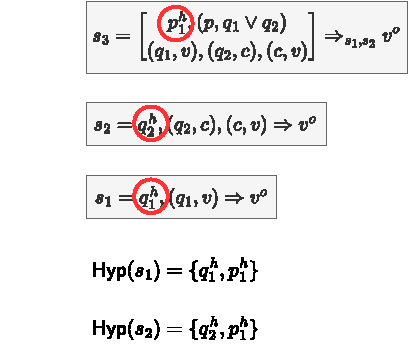
\includegraphics[scale=1.2]{pic/Hyp function.pdf}
	\end{figure}
\end{frame}

\begin{frame}[label={sec:org013357e},fragile]{}

\(s\) \alert{defeats} \(s'\) iff
\begin{enumerate}
	\item \(\mathsf{Con}(s) = \neg(\phi,\psi)\) for some \((\phi,\psi) \in \mathsf{Norms}(s'),\)
	\item $\mathsf{Hyp}(s)\subseteq\mathsf{Hyp}(s'),$
	\item $\forall t\in\mathsf{Arg}$, if $(\varphi,\psi)\in\mathsf{Norms}(t)$, then \(\mathsf{Hyp}(t)\not\subset\mathsf{Hyp}(s).\)
\end{enumerate}
Or, 

\(\exists t \in \mathsf{Sub}(s')\) such that \(s\) defeats \(t\).


\end{frame}

\begin{frame}
	Why do we need Condition 3?
	
Condition 3:	$\forall t\in\mathsf{Arg}$, if $(\varphi,\psi)\in\mathsf{Norms}(t)$, then \(\mathsf{Hyp}(t)\not\subset\mathsf{Hyp}(s).\)
\end{frame}

\begin{frame}
	\begin{figure}
		\centering
		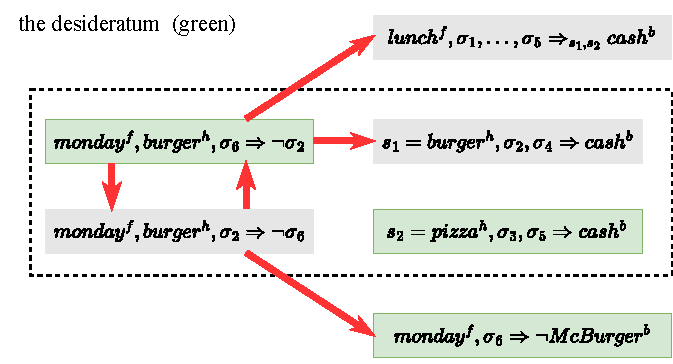
\includegraphics[scale=1]{pic/figure2.pdf}
	\end{figure}
	
	Hypothetical arguments are denoted by the dashed-line.
\end{frame}

\begin{frame}
	\begin{figure}
		\centering
		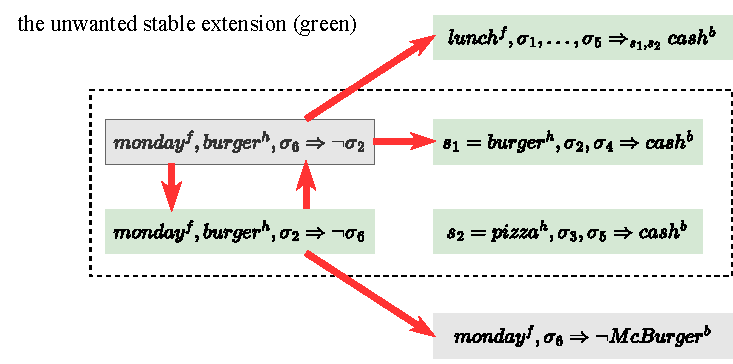
\includegraphics[scale=1]{pic/figure1.pdf}
	\end{figure}
	
	Hypothetical arguments are denoted by the dashed-line.
\end{frame}

\begin{frame}
	The consequence relation is defined on the basis of the conclusions of arguments with no hypothetical assumptions. 
	
	Let \(\mathscr{E}\) be a set of argument. We define 
	$\mathsf{Real}(\mathscr{E})=\{\Gamma\Rightarrow\Sigma\mid \exists a=\Gamma\Rightarrow_{\Theta}\Sigma\in \mathscr{E}\text{ and } \mathsf{Hyp}(a)=\emptyset\}$.
\end{frame}

\begin{frame}
	Let $\mathcal{K}=\langle\mathcal{F},\mathcal{N}\rangle$ be a knowledge base. 
	
	Let $\langle\mathsf{Arg}^d,\mathsf{Att}^d\rangle$ be the $\mathscr{A\!F}^d(\mathcal{K})$ induced by $\mathsf{HDAC}$. 
	
	Let $\langle\mathsf{Arg},\mathsf{Att}\rangle$ be the $\mathscr{A\!F}(\mathcal{K})$ induced by $\mathsf{DAC}$.
	
	\pause
	\vspace{9pt}
	\textbf{Q1}: For every $\mathscr{E}\subseteq\mathsf{Arg}$ that is a stable extension of $\mathsf{Arg}$, does there always exist a stable extension $\mathscr{E}^d\subseteq\mathsf{Arg}^d$ such that $\mathsf{Real}(\mathscr{E}^d)\subseteq\mathscr{E}$?

	\pause
	\vspace{9pt}
	\textbf{Q2}: For every $\mathscr{E}^d\subseteq\mathsf{Arg}^d$ that is a stable extension of $\mathsf{Arg}^d$, does there always exist a stable extension $\mathscr{E}\subseteq\mathsf{Arg}$ such that $\mathsf{Real}(\mathscr{E}^d)\subseteq\mathscr{E}$?
\end{frame}

\begin{frame}
	For both question: \textbf{NO}.
	
	Here we only show the counterexample for Q1.
	
	Consider the following knowledge base.
	
	\begin{figure}[!h]
		\centering
		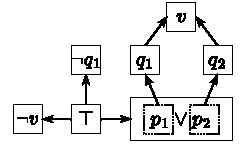
\includegraphics[scale=1.2]{pic/example1.pdf}
	\end{figure}
\end{frame}

\begin{frame}
	\begin{figure}[!h]
		\centering
		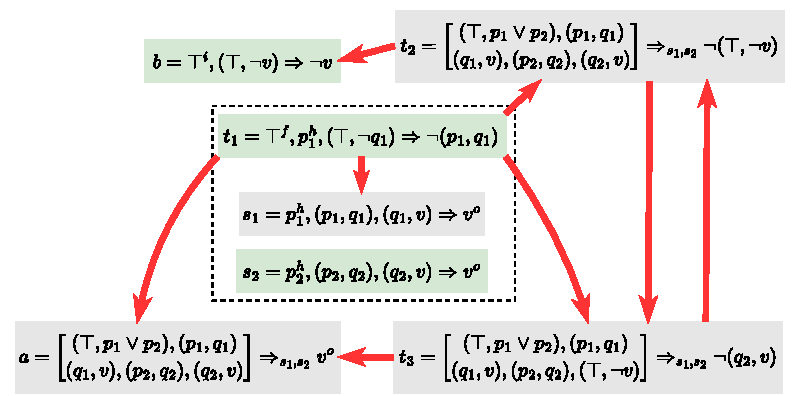
\includegraphics[scale=0.87]{pic/example1_argument.pdf}
	\end{figure}
	
	There exists an stable extension $\mathscr{E}\subseteq\mathsf{Arg}$ concluding $v$, but there is only one stable extension $\mathscr{E}^d\subseteq\mathsf{Arg}^d$concluding $\neg v$.
\end{frame}

\end{comment}
\begin{frame}[label={sec:orgcbf8e3f}]{}
Thank you (and our collaborators)! :-)

\vspace{2cm}

\begin{columns}
\begin{column}{.3\columnwidth}
\begin{center}

\includegraphics[width=.9\textwidth]{./images/logo-lodex.png}
\end{center}
\end{column}
\begin{column}{.3\columnwidth}
\begin{center}

\includegraphics[width=.9\textwidth]{images/rrs-logo.png}
\end{center}
\end{column}
\begin{column}{.3\columnwidth}
\begin{center}

\includegraphics[width=.9\textwidth]{images/logo-lpai.png}
\end{center}
\end{column}
\end{columns}
\end{frame}
\end{document}

